\documentclass[11pt]{article}
\usepackage[utf8]{inputenc}
\usepackage[english,italian]{babel}
\usepackage{graphicx}
\usepackage{hyperref}
\usepackage{verbatim}
\usepackage{mathtools}
\usepackage{booktabs}
\usepackage{comment}


\usepackage[backend=biber]{biblatex}
\addbibresource{bibliografia.bib}




\begin{document}

\title{Simulazione di un ecosistema Preda-Predatore}

\author{Mattia Marchi 817587 \\
Lorenzo Tomasoni 829906 }

\maketitle

\vspace{5cm}

\begin{center}
\Large{Sistemi Complessi: Modelli e Simulazione}

\vspace{4cm}

\large{Università degli Studi Milano- Biccoca \\
Dipartimento di Informatica, Sistemistica e Comunicazione \\
Anno Accademico 2020-2021}
\end{center}

\newpage

\begin{abstract}
    In questo documento viene illustrato un modello di simulazione multi-agente di un ecosistema naturale, caratterizzato dalla presenza di prede e predatori. Dapprima viene presentata una panoramica relativa allo stato dell'arte della simulazione dei sistemi complessi in generale e dei modelli presenti in letteratura dedicati alla simulazione di sistemi preda-predatore. In seguito viene illustrato il modello realizzato, la validazione e l'analisi dei risultati ottenuti dalla simulazione. 
\end{abstract}

\newpage

\tableofcontents


\newpage

\section{Introduzione}
Il termine ecosistema naturale identifica una comunità di organismi che vivono in congiunzione con i componenti non viventi che si collocano nell'ambiente che li circonda, interagendo con essi e comportandosi come un sistema. In particolare, l'european environment agency definisce un ecosistema naturale come una particolare categoria di ecosistema dove l'impatto umano non ha avuto una influenza maggiore di quello di qualsiasi altra specie autoctona e non ha influenzato la struttura dell'ecosistema dalla rivoluzione industriale. L'impatto umano esclude cambiamenti di proporzioni globali, come il cambiamento climatico dovuto al riscaldamento globale \cite{EEA}.

L'obiettivo del progetto è quello di realizzare una simulazione basata su agenti al fine di simulare il comportamento di un piccolo ecosistema naturale, costituito da una specie di predatori (volpi), una specie di prede (conigli), da alcune specie (non distinte) di vegetali e infine, da alcuni specchi d'acqua. Entrambe le specie animali presenti nell'ecosistema devono soddisfare alcuni bisogni: fame, sete e necessità di riprodursi. Per soddisfare il bisogno di cibarsi le volpi si cibano dei conigli e i conigli si cibano dei vegetali ed entrambi saziano la propria sete bevendo dai piccoli specchi d'acqua presenti nell'ambiente. Ogni singolo individuo è caratterizzato da alcune specifiche caratteristiche genetiche quali: soglia della fame, velocità di movimento, velocità di punta, raggio di visione, necessità di accoppiarsi e così via. Ogni individuo è in grado di riprodursi e lo potrà fare solamente quando ne sente la necessità e incontra un altro individuo della stessa specie e di sesso opposto che ha altrettanta necessità di riprodursi. Ogni individuo che nasce in seguito all'accoppiamento erediterà i geni dai genitori.  

Il fine del lavoro è quello di valutare come, al variare di alcuni parametri quali numero di prede, numero di predatori, stagione e parametri genetici degli individui il sistema evolve nel tempo. Oltre a ciò, l'obiettivo è quello di introdurre ad un certo punto del periodo di simulazione una variazione genetica negli individui in modo tale da valutare come questa possa avere effetto sull'equilibrio (o meno) instauratosi nell'ecosistema. 


\newpage
\section{Panoramica sugli ecosistemi naturali}
\subsection{Cos'è un ecosistema naturale}
Il termine ecosistema venne per la prima volta usato in una pubblicazione dall'ecologista inglese Arthur Tansley nel 1935.\cite{WikiEcosystem}
Un ecosistema\cite{Vedantu}, come già accennato nelle precedentemente, può essere definito come una comunità dove esseri viventi di specie differenti coesistono nello stesso ambiente fisico e interagisco vicendevolmente in modo da sviluppare un ciclo di vita e facilitare il flusso di energia e nutrienti. 
Due sono le componenti di un sistema di questo tipo: quella biotica e quella abiotica. La prima comprende piante, animali e altri organismi viventi. Elementi fisici quali temperatura, minerali, piogge e umidità definiscono la componente abiotica di un ecosistema. 

Esistono due tipi di ecosistemi: quelli naturali e quelli artificiali. La prima categoria riguarda quegli ecosistemi che si sviluppano naturalmente e che possono svilupparsi e sopravvivere senza l'intervento umano. Ne sono esempi le foreste, le montagne, i fiumi, i prati e così via. Gli ecosistemi artificiali \cite{ArtificialEcosystems}, invece, hanno caratteristiche in comune con quelli naturali, ma sono creati e mantenuti dagli essere umani. Essi sono più semplici rispetto a quelli naturali e sono quelli che più comunemente circondano l'esistenza umana. 

L'ecosistema che il progetto si pone l'obiettivo di simulare è un semplice ecosistema naturale costituito da tre sole specie viventi, volpi rosse, conigli selvatici e carote e da una componente abiotica, l'acqua. La quantità di acqua presente nell'ecosistema simulato dipende dalla stagione: durante i mesi invernali e autunnali le piogge sono più frequenti e quindi l'acqua abbonderà maggiormente nell'ambiente, viceversa, nei mesi più caldi l'acqua tenderà a scarseggiare. 

\subsubsection{La volpe rossa}
\label{volpe}
La volpe rossa (\emph{vulpes vulpes}) è la più grande delle volpi e il carnivoro più largamente diffuso, essendo presente in tutto l'emisfero boreale dal circolo polare artico all'Africa settentrionale, il nord America e l'Eurasia \cite{WikiVolpe}.
Questi animali possono misurare dai 75 ai 140 cm, per un peso che varia tra i 3 e gli 11 Kg. Il colore varia tra il giallo e il marrone e spesso è rossiccio. 

La specie ebbe origine da antenati più piccoli in Eurasia durante il Villafranchiano medio \cite{KurtenBjorn} e colonizzò il Nord America poco dopo la glaciazione di Wisconsin.\cite{Kurten1980Sep}

La volpe rossa vive generalmente in coppia con i cuccioli, ma talvolta è possibile osservare degli esemplari che vivono solitari oppure in gruppi di 4-6 adulti. Generalmente le volpi rosse cacciano in modo solitario e difendono il proprio territorio da sole durante l'estate e in coppia durante l'inverno. 

L'alimentazione della volpe rossa, nonostante sia classificato come animale carnivoro, comprende sia animali che vegetali. La dieta di questo animale è basata su una grande quantità di specie dagli invertebrati ai piccoli mammiferi, uova rettili e piccoli anfibi. Tra i vegetali, la volpe rossa si ciba di vari tipi di frutti di bosco. In particolare, la volpe rossa caccia i conigli appostandosi in modo furtivo e silenzioso per poi balzare tramite un rapido scatto sulla preda. 

Il periodo degli amori è molto variabile e cambia secondo la latitudine: in Italia ha luogo in inverno, tra dicembre e febbraio. I parti avvengono generalmente tra marzo e aprile. La femmina, dopo una gestazione di 7 settimane, partorisce in media da 3 a 5 piccoli, che vengono allattati per un mese. Le volpi si riproducono una sola volta all'anno. 

In natura, le volpi rosse possono raggiungere l'età di 12 anni.

\begin{figure}[h]
    \centering
    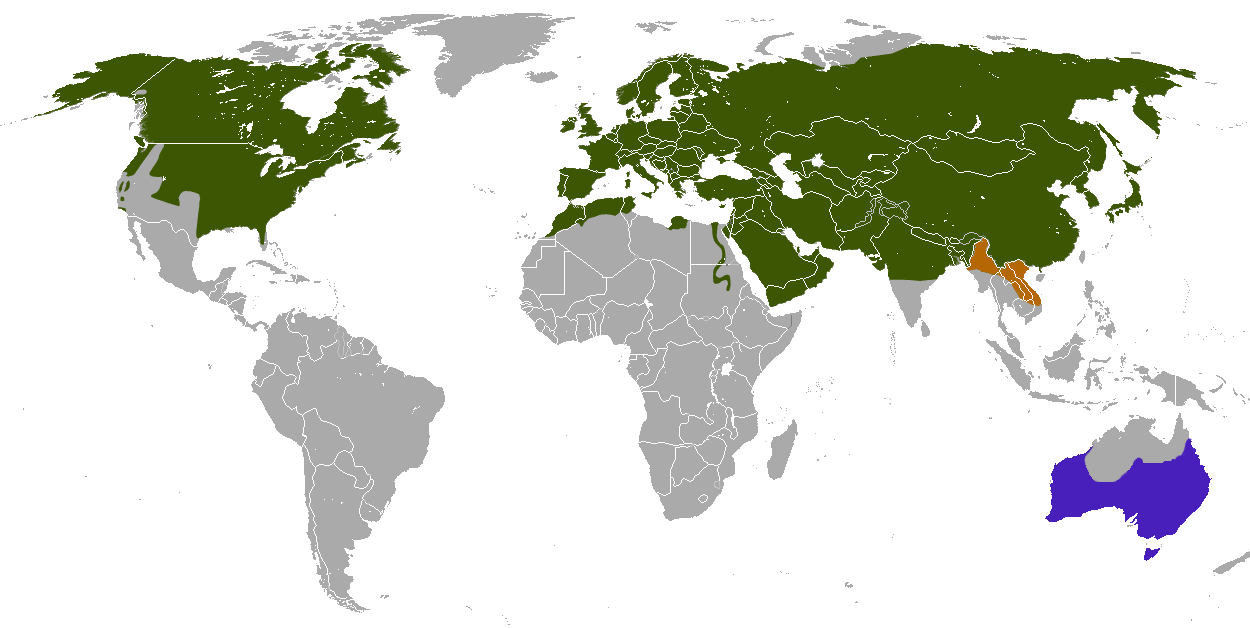
\includegraphics[scale = 0.3]{ArealeDellaVolpe.png}
    \label{figArealeVolpe}
    \caption{Areale della volpe. Le zone in verde indicano le aree dove la volpe è nativa, quelle blu dove è introdotta e quello in arancione dove la presenza della volpe è dubbia. }
\end{figure}

Osservazioni sul campo\cite{RedFox} suggeriscono che le volpi siano miopi; possono attraversare la vegetazione senza incidenti, ma si avvicineranno agli oggetti fermi entro pochi metri a meno che un altro senso (come l'udito o l'olfatto) non le avvertano del pericolo o l'oggetto si muova. Huw Lloyd, nel proprio libro intitolato The red fox \cite{Zimen1980}, ha presentato alcuni diagrammi del campo visivo della volpe e, sulla base di questi disegni, è risultato che le volpi hanno un campo visivo di circa 260 gradi, con un punto cieco che copre circa 100 gradi direttamente dietro la loro testa e un sovrapposizione dei campi degli occhi destro e sinistro di circa 40 gradi. Il grado di sovrapposizione viene chiamato visione binoculare e consente agli animali di giudicare le distanze.
Confrontando questo aspetto con i conigli, essi hanno un campo visivo di circa 360 gradi (sono ciechi solo in un'area di 10 gradi direttamente davanti al loro naso), ma hanno una sovrapposizione binoculare di soli 20 gradi circa; questo li rende bravi a individuare le volpi che si avvicinano di soppiatto, ma non sono in grado di dire in modo efficace quanto sia lontano il pericolo. Al contrario, gli esseri umani possono vedere oggetti all'interno di un arco orizzontale di circa 180 gradi direttamente di fronte ad essi senza muovere gli occhi o la testa, ma circa 140 gradi di questo campo sono una sovrapposizione binoculare, il che ci rende molto bravi a giudicare la distanza.

Le volpi hanno due orecchie altamente mobili, che possono essere mosse indipendentemente l'una dall'altra. Esse possono ruotare ciascun orecchio di circa 150 gradi in un'unica direzione, l'orecchio destro ruota in senso orario e l'orecchio sinistro in senso antiorario, per captare i suoni di lato e dietro di loro. L'udito della volpe è molto sensibile ai suoni a bassa frequenza, come i fruscii emessi dalle prede. 

Per quanto concerne l'olfatto, la volpe rossa sfrutta questo senso non solo per identificare le prede, ma anche per comunicare con i propri simili e delimitare il proprio territorio.



\subsubsection{Il coniglio selvatico}
\label{coniglio}
Il coniglio selvatico\cite{WikiConiglio} europeo(Oryctolagus cuniculus) è un mammifero della famiglia dei leporidi, diffuso in gran parte dell'Europa (dal Portogallo alla Polonia, in Gran Bretagna e in alcune parti della Norvegia, Svezia e Ucraina), oltre al Nord Africa. Inoltre, i conigli selvatici sono stati introdotti in  Australia, Nuova Zelanda, Cile ed in numerose isole. 

\begin{figure}[h]
    \centering
    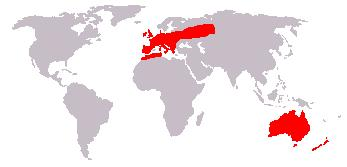
\includegraphics[scale = 1]{ArealeDelConiglioSelvatico.jpeg}
    \label{figArealeConiglio}
    \caption{Areale del coniglio selvatico.}
\end{figure}

Il coniglio selvatico predilige ambienti aperti, con clima secco e mite, ad altitudine non troppo elevata: il suolo dev'essere soffice o sabbioso, in modo da permettere all'animale di scavarsi la tana. Misura fino a 45 cm di lunghezza, per un peso che raggiunge i 2,5 kg: i maschi sono generalmente più grossi e robusti delle femmine. Si tratta di animali principalmente notturni e fortemente gregari, che possono vivere in colonie di grandezza direttamente proporzionale alla disponibilità di cibo. Una colonia tipo è composta da una decina di individui, senza distinzione di sesso. 

I conigli selvatici son animali erbivori che si nutrono di diversi tipi di vegetali, dall'erba alle foglie e le radici. 

I conigli sono famosi per la propria capacità riproduttiva: la femmina va infatti in estro ogni 21 giorni (anche se l'ovulazione è indotta dall'accoppiamento) e tende a riprodursi durante i primi mesi dell'anno, anche se in condizioni favorevoli può allevare i piccoli durante tutto l'anno al ritmo di una cucciolata al mese. Tuttavia, in condizioni di stress essa può abortire spontaneamente o riassorbire gli embrioni.
Le modalità di corteggiamento del coniglio selvatico sono tuttavia state poco studiate: pare che i maschi di rango più alto abbiano degli harem (poliginia), mentre quelli di ranghi inferiori tendano a formare delle coppie stabili (monogamia).

La gestazione dura un mese, al termine del quale vengono dati alla luce dai 3 ai 14 cuccioli. La femmina del coniglio può tornare a riprodursi appena dopo il parto\cite{Gattoni2019Apr}.  La speranza di vita di questi animali è di circa 9 anni, anche se in generale il 90\% degli esemplari muore prima di raggiungere l'anno d'età, a causa della forte pressione dei predatori. 


\subsection{La teoria della selezione naturale di Darwin}
Uno degli obiettivi del progetto è stato quello di simulare come l'evoluzione genetica e l'adattamento rispetto alle condizioni dell'ambiente influenzino la competizione tra le prede e i predatori. 

Il concetto di selezione naturale è stato introdotto per la prima volta dal biologo, naturalista e antropologo britannico Charles Darwin nel 1859 nella famosa opera \emph{L'origine delle specie}\cite{darwin1859}. Si tratta di un meccanismo alla base dell'evoluzione, secondo il quale il numero di individui che dimostrano di avere caratteristiche che si adattano in modo ottimale all'ambiente in cui vivono tende a aumentare in modo progressivo nel lungo periodo.
Gli individui di una specie si distinguono per alcune caratteristiche genetiche. La teoria della selezione naturale afferma che tale variabilità è causata da mutazioni genetiche casuali, ovvero non causate dall'adattamento degli individui all'ambiente, ma generate in modo casuale. Con il passare del tempo, vengono selezionate (ovvero favorite) quelle mutazioni che permettono agli individui di adattarsi meglio all'ambiente in cui vivono. 

Gli individui che si adattano meglio a un certo habitat hanno la possibilità di procacciarsi più facilmente il cibo e si accoppieranno più facilmente rispetto agli altri individui della stessa specie che non presentano tali caratteristiche. Quindi si può dire che è l'ambiente a selezionare le mutazioni in base a come esse permettano l'adattamento degli individui. I geni che fanno si che l'individuo si adatti bene all'ambiente verranno trasmessi di generazione in generazione, mentre quelli inutili o dannosi vengono scartati. Questo porta all'evoluzione della specie che svilupperà caratteristiche che la rendono adatta a vivere e sopravvivere nell'ambiente. 

Uno degli esempi più classici quando si parla di selezione naturale è quello relativo al collo delle giraffe. Nel corso di centinaia di migliaia di anni le mutazioni genetiche fecero in modo che alcuni individui di giraffe avessero un collo più lungo. Questa caratteristica si rivelò molto vantaggiosa perché permise a questi individui di raggiungere con agilità le foglie degli alberi più alti. In situazioni di scarsità di cibo questa caratteristica si rivelò determinante: gli individui con il collo lungo avevano maggiore probabilità di sopravvivere, di raggiungere l'età della riproduzione e di conseguenza di riprodursi e di trasmettere i propri geni (e di conseguenza anche la peculiarità del collo lungo) alle generazioni successive. 

I principi generali su cui si basa la teoria della selezione naturale sono i seguenti:
\begin{itemize}
    \item \textbf{principio della variazione}: tra gli individui di una stessa popolazione esiste una variabilità di caratteri;
    \item \textbf{principio dell'adattamento}: gli individui che meglio si adattano all'ambiente hanno dei caratteri che offrono un vantaggio in termini di sopravvivenza e di riproduzione;
    \item \textbf{principio dell'ereditarietà}. Si tratta del principio secondo il quale le caratteristiche trasmissibili ai discendenti per mezzo della riproduzione sono localizzate all'interno dei geni degli individui. 
\end{itemize}

Il processo di selezione naturale è un fattore che sta alla base del processo di adattamento delle specie e che quindi concorre, insieme alle mutazioni genetiche e alla deriva genetica, all'evoluzione delle stesse.

La selezione naturale è anche alla base della della speciazione, ovvero quel processo che porta alla nascita di nuove specie. Questo fenomeno in genere si verifica quando le popolazioni della stessa specie sono divise da barriere geografiche e quindi vengono sottoposte a pressioni selettive differenti. Questo produce differenze nella loro struttura anatomica. Nel lungo periodo le differenze accumulate tra gli individui delle popolazioni diventano talmente grandi che essi non possono più accoppiarsi e quindi dalla stessa specie se ne originano di nuove. 

\section{Stato dell'arte}
\subsection{Sistemi complessi}
In letteratura esistono svariate definizioni, più o meno formali, di sistema complesso. In via del tutto generale, possiamo definire un sistema complesso come un sistema altamente strutturato, dinamicamente in evoluzione nel corso del tempo, il cui funzionamento è spesso complesso da spiegare o comprendere e in cui si verificano spesso interazioni multiple tra differenti componenti del sistema stesso. Diverse sono le caratteristiche tipiche dei sistemi complessi: 
\begin{itemize}
    \item i sistemi complessi sono spesso formati da elementi in continua interazione. Spesso questi elementi prendono il nome di agenti;
    \item la \textbf{non linearità}. Spesso emerge che nei sistemi complessi non esiste un rapporto lineare tra l'input e l'output.
    \item Possibilità di evolvere ed adattarsi nel tempo. 
    \item Robustezza e plasticità dei sistemi. 
\end{itemize}
Oltre ai sistemi complessi, possiamo definire altre due categorie di sistemi: i sistemi semplici e quelli complicati. La categoria dei sistemi semplici comprende quei sistemi le cui relazioni causa-effetto sono ben note e documentate, oltre che prevedibili e ripetitive. Si può affermare che i sistemi semplici sono sistemi noti e conosciuti. Ne è un esempio la bicicletta. Un sistema complicato invece, è un sistema molto simile dal punto di vista delle relazioni causa-effetto ai sistemi semplici; la differenza risiede nel fatto che i sistemi complicati sono a più ampia scala e richiedono expertise specializzate. Sono sistemi che potremmo definire conoscibili e ne sono esempi le macchine, i razzi spaziali, i treni e così via. Infine, i sistemi complessi si differenziano dalle altre due categorie di sistemi a causa del fatto che le relazioni causa-effetto possono essere apprese in retrospettiva, ma difficilmente risultano essere riproducibili o predicibili. Questa categoria di sistemi è analizzabile seguendo l'approccio della simulazione. Ne sono esempi gli organismi viventi, il sistema nervoso umano e, ovviamente, gli ecosistemi naturali che sono oggetto del progetto descritto in questo documento. 
\subsection{Simulazione di sistemi complessi}
Come già affermato precedentemente, i sistemi complessi sono difficili da studiare e analizzare con un approccio teorico, è quindi opportuno utilizzare un approccio basato sulla simulazione. I modelli e le simulazioni di vario tipo sono strumenti per rapportarsi con la realtà. Gli esseri umani hanno sfruttato i modelli e la simulazione per prendere decisioni, per meglio comprendere i fenomeni naturali, per validare teorie oppure per valutare l'impatto di un cambiamento. Anche migliaia di anni fa, costruzioni, macchine e navi venivano prima testati come modelli in scala ridotta prima di essere realizzati nella loro forma finale. Nel momento in cui gli scienziati identificano principi generalizzabili, essi costruiscono modelli, che vengono usati per simulare e investigare nuove possibilità che potrebbero condurre a nuove opportunità tecnologiche. I modelli possono presentarsi in varie forme: schemi, diagrammi, costrutti logici oppure sotto forma di software. I modelli realizzati con questo ultimo approccio permettono di realizzare una simulazione del comportamento dinamico del sistema in oggetto \cite{ModelingAndSimulation}.

Gli scopi per cui si fa simulazione sono vari e possono essere riassunti nei seguenti punti:
\begin{itemize}
    \item Valutare piani e progetti operativi senza la necessità di metterli in atto nel mondo reale. Questo punto è molto importante perché attraverso la simulazione è possibile evitare di mettere in pratica un piano operativo per poi accorgersi che non può essere portato a termine in modo corretto. Questo permette di risparmiare risorse e fatica.
    \item Valutare teorie e modelli. Questo significa che la simulazione permette di comprendere meglio il sistema che stiamo studiando, valutandone le relazioni di causa-effetto che lo fanno evolvere in modo dinamico.
    \item Osservare un sistema che non è ancora stato realizzato nel mondo reale e che pertanto non è osservabile. Questa situazione si può verificare nel momento in cui il sistema è in via di sviluppo.
\end{itemize}
In estrema sintesi, è possibile definire la simulazione come la disciplina che consente di definire un modello della realtà che consente di valutare e prevedere lo svolgersi dinamico di una serie di eventi o processi susseguenti all'imposizione di certe condizioni da parte dell'analista o dell'utente \cite{WikiSimulazione}.

Come per tutti gli strumenti scientifici, anche per fare simulazione non esiste un unico approccio. Il primo approccio usato per fare simulazione è quello macroscopico. Utilizzando questo approccio vengono specificati dei vincoli globali, rappresentati sotto forma di equazioni. Un esempio è il vincolo della conservazione della massa che impone che qualunque cosa succeda nel sistema la quantità di massa totale dovrà mantenersi costante nel tempo. Nei modelli macroscopici vengono stilate delle equazioni differenziali che indicano come variano le quantità aggregate nel corso del tempo. Si assume che gli individui siano tutti uguali e abbiano lo stesso comportamento e lo stesso atteggiamento. Lo svantaggio di questo approccio è che rende difficile catturare tutti gli aspetti della dinamica del gruppo di agenti che compongono il sistema. L'approccio macroscopico è particolarmente indicato per problemi di ottimizzazioni in contesti specifici. Per esempio, il metodo macroscopico potrebbe rivelarsi utile per simulare l'evacuazione di un edificio e per verificare se tutte le persone all'interno dell'edificio sono in grado di evacuare in meno di 10 minuti.
Uno degli esempi più famosi di modelli di simulazione macroscopici è il modello di Lotka-Volterra, descritto \hyperref[sec:LV]{in una delle prossime sezioni}. 

L'approccio alternativo prende il nome di simulazione basata sugli agenti. Con questa metodologia l'unità analitica è costituita dal singolo individuo (che prende appunto il nome di agente) e non più le variabili aggregate come nell'approccio macroscopico. Il vantaggio di questo approccio sta nel fatto che i risultati dovrebbero evidenziare esattamente le stesse dinamiche descritte dai modelli macroscopici, oltre ad altre informazioni aggiuntive relative, per esempio, all'aspetto spaziale. Per esempio, nel contesto di un ecosistema naturale, alcuni modelli microscopici mi permettono di comprendere con un buon livello di confidenza dove si collocano i predatori e quali percorsi tendono a seguire. L'aspetto negativo riguarda il fatto che per realizzare un modello microscopico è necessario conoscere alcuni aspetti aggiuntivi del sistema e degli agenti che lo compongono. Per esempio, sempre prendendo in considerazione il modello dell'ecosistema naturale, è necessario conoscere come sono fatti i predatori, quali sono le loro caratteristiche, come cacciano, quali bisogni hanno e per le prede conoscere di cosa si cibano, come scappano o si nascondono dai predatori e così via. 

A prescindere dall'approccio che si usa, il ciclo di vita di un modello di simulazione è ben delineato. Infatti, per effettuare la corretta simulazione di un sistema complesso in generale si segue il ciclo di sviluppo riportato in figura \ref{figCicloSviluppo}.

Come si vede dall'immagine, le fasi dello sviluppo di una simulazione di un sistema complesso sono le seguenti: 
\begin{itemize}
    \item Definizione di un sistema target di riferimento, derivante dal processo interdisciplinare di analisi del fenomeno che si vuole studiare attraverso la simulazione. 
    \item Eseguire un'operazione di modellazione e progettazione di un modello concettuale e di un simulatore del sistema in esame. 
    \item Esecuzione di simulazioni. Questo passaggio permette di acquisire una grande quantità di dati che risultano essere particolarmente utili nella fase successiva.
    \item Analisi dei risultati e validazione. In quest'ultima fase si sfruttano i dati raccolti dalle simulazioni effettuate e li si confrontano con i dati reali collezionati all'inizio del ciclo per la realizzazione del sistema target. Se i risultati della simulazione coincidono con le dinamiche osservate nel sistema reale (ovvero se il ciclo commuta), è possibile sfruttare il modello realizzato per fini esplicativi oppure predittivi; viceversa se dal modello sviluppato si ottengono dati che non coincidono con le osservazioni raccolte è necessario ripetere il ciclo e adattare il modello, sistemandone alcuni aspetti. In caso il ciclo dovesse commutare non si può avere la certezza di aver colto tutti gli aspetti essenziali e rilevanti del mondo reale, è unicamente possibile affermare che le teorie generate dal modello non sono contraddette dalla simulazione. 
\end{itemize}

\begin{figure}
    \centering
    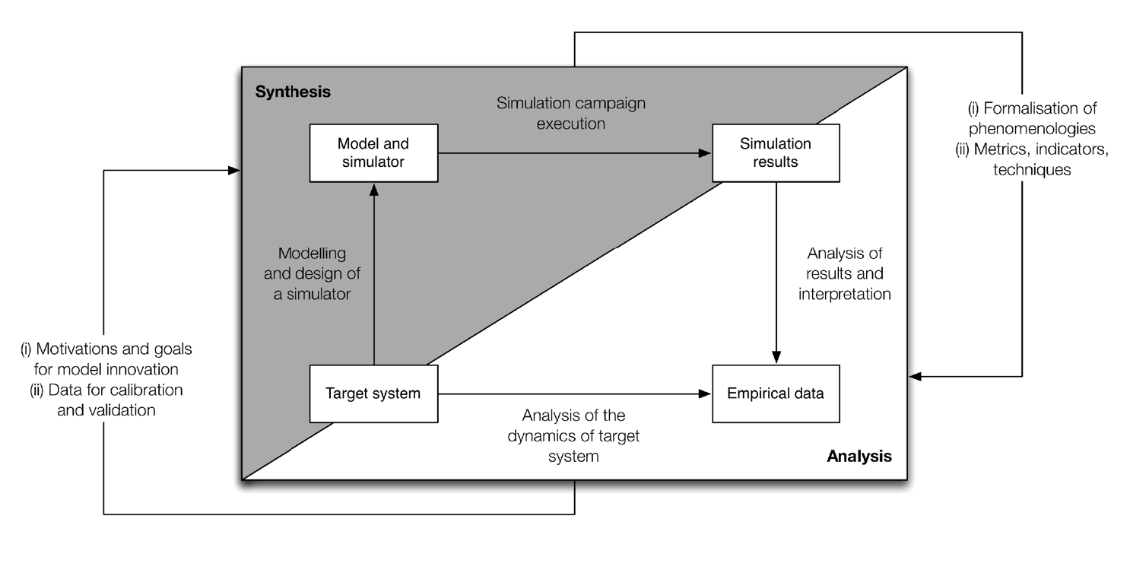
\includegraphics[scale = 0.6]{cicloSviluppoSimulazione.png}
    \label{figCicloSviluppo}
    \caption{Schema che rappresenta il ciclo di sviluppo di una simulazione di un sistema complesso}
\end{figure}

\subsection{Il modello Lotka-Volterra}
\label{sec:LV}
Il modello di Lotka-Volterra, noto anche come equazioni o modello preda-predatore, è il modello matematico più noto di analisi dei sistemi di tipo preda-predatore. Questo modello è stato proposto in modo indipendente dal matematico americano Alfred J. Lotka nel 1925 e dal fisico e matematico italiano Vito Volterra nel 1926. 

Il modello venne inizialmente proposto da Alfred J. Lotka nella teoria delle reazioni chimiche autocatalitiche pubblicata nel 1910 \cite{Goel}. Successivamente dieci anni più tardi, Lotka estese il proprio modello, grazie anche al contributo del matematico sovietico Andrey Kolmogorov, a sistemi organici, utilizzando come esempio piante e specie di animali erbivori \cite{Lotka1920}. Infine, nel 1925 Lotka sfruttò il modello per analizzare l'interazione tra prede e predatori in un ambiente naturale\cite{Lotka1925}. L'anno successivo Vito Volterra si interessò allo stesso modello, voleva rispondere alla questione sollevata dal biologo Umberto d'Ancona\cite{Bacaer}. Egli aveva osservato che le percentuali di pesci cacciatori catturati dai pescatori erano aumentate durante la prima guerra mondiale. Questa osservazione lo stupì dato che durante gli anni di guerra la pesca venne praticata in misura molto minore rispetto agli anni precedenti. Volterra sviluppò il proprio modello in modo del tutto indipendente da Lotka e lo utilizzò per spiegare questo apparente paradosso. 

Il modello di Lotka-Volterra\cite{Artioli} descrive la dinamica di interazione fra due specie che convivono in uno stesso ambiente e sono in interazione tra di loro, definendo le seguenti ipotesi, che non sono necessariamente realizzabili in natura: 
\begin{enumerate}
    \item Le prede hanno sempre a disposizione una quantità ampia di cibo a disposizione. In altre parole, questo significa che le prede non potranno mai morire a causa della scarsità di cibo. 
    \item I predatori si cibano esclusivamente delle prede. 
    \item Il tasso di crescita delle popolazioni di entrambe le specie è proporzionale rispetto al numero di individui che compongono popolazioni stesse.
    \item L'ambiente, con il trascorrere del tempo, non evolve a favore di nessuna delle sue specie e i cambiamenti genetici sono irrilevanti. 
    \item La necessità di cibarsi dei predatori è limitata. 
\end{enumerate}

Sotto queste ipotesi, il modello di Lotka-Volterra prende la forma di un sistema di equazioni differenziali non lineari del primo ordine:
\[
\label{eqn:modelloGenerale}
\left\{
\begin{array}{cc}
\frac{dx}{dt}=\alpha x(t) - \beta x(t)y(t)\\
\frac{dx}{dt}=\delta x(t)y(t) - \gamma y(t)
\end{array}
\right.
\]

Dove: 
\begin{itemize}
    \item x(t) e y(t) rappresentano rispettivamente il numero di prede e predatori che popolano il sistema al tempo t.
    \item I parametri $\alpha$ e $\gamma$ indicano il tasso di crescita rispettivamente delle prede e dei predatori. In altre parole, indicano la differenza tra il tasso di nascita e il tasso di morte delle due specie.
    \item Il parametro negativo $-\beta$ indica come diminuiscono le prede in funzione dei predatori.
    \item Il parametro positivo $\delta$ indica come crescono i predatori in funzione delle prede. 
\end{itemize}

\noindent Nel caso specifico di un sistema che presenti solo prede, ricordando che esse hanno la possibilità di riprodursi senza limiti, l'unica cosa che può farne diminuire il numero sono i predatori.  
In questa situazione il sistema si può tradurre in un'unica equazione, che assume la seguente forma: 
\[
    \frac{dx}{dt} = \alpha x(t) 
\]
Anche in questo caso il parametro positivo alpha indica il tasso di crescita delle prede. 
La soluzione a tale equazione è 
\begin{equation}\label{eqn:soloPrede}
    x(t) = x(0)e^{\alpha t}
\end{equation}

\noindent Dove x(0) rappresenta il numero di prede presenti nel sistema al tempo 0.

\noindent Analizzando il grafico della funzione \eqref{eqn:soloPrede} riportato in figura \ref{figPlotLotkaVolterraSoloPrede}, è possibile notare che la funzione è monotona crescente. Questo implica che le prede continueranno a crescere in numero dato che l'unico fattore che potrebbe limitarne la crescita è rappresentato dai predatori. 

\begin{figure}[h]
    \centering
    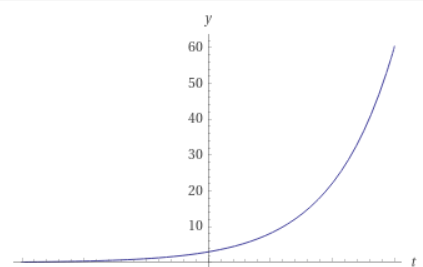
\includegraphics[scale = 1]{plotSoloPrede.PNG}
    \label{figPlotLotkaVolterraSoloPrede}
    \caption{Grafico della funzione \eqref{eqn:soloPrede} fissati i parametri x(0) e $\alpha$ rispettivamente a 3 e 2}
\end{figure}

\noindent Studiando invece, il caso specifico in cui il sistema è abitato esclusivamente da predatori, il sistema di equazioni differenziali si riduce, anche in questo caso, ad una sola equazione che assume la seguente forma: 

\[
    \frac{dy}{dt} = -\gamma y(t) 
\]

Anche in questo caso il parametro negativo $-\gamma$ indica il tasso di morte dei predatori. 
Risolvendo l'equazione, otteniamo il seguente risultato:
\begin{equation}\label{eqn:soloPredatori}
    y(t) = y(0)e^{-\gamma t}
\end{equation}

\noindent Dove y(0) rappresenta il numero di predatori che popolano il sistema al tempo 0.

\noindent Analizzando il grafico della funzione \eqref{eqn:soloPredatori} riportato in figura \ref{figPlotLotkaVolterraSoloPredatori}, è possibile notare che la funzione è monotona decrescente. Questo implica che i predatori continueranno a diminuire in numero fino a estinguersi completamente. 

\begin{figure}[h]
    \centering
    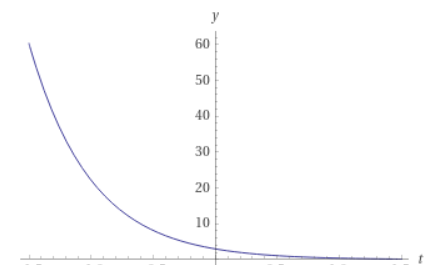
\includegraphics[scale = 1]{plotSoloPredatori.PNG}
    \label{figPlotLotkaVolterraSoloPredatori}
    \caption{Grafico della funzione \eqref{eqn:soloPredatori} fissati i parametri y(0) e $\gamma$ rispettivamente a 3 e 2}
\end{figure}

Il modello Lotka-Volterra generale, descritto dal sistema \ref{modelloGenerale} presente il seguente andamento: 
\begin{itemize}
    \item Il numero di prede tende a crescere fintantoché il numero di predatori rimane basso;
    \item Al crescere delle prede, cresce anche il numero di predatori;
    \item Quando il numero di predatori è elevato e superiore rispetto a una certa soglia, il numero di prede tende a calare;
    \item Il diminuire delle prede viene accompagnato dalla contestuale diminuzione del numero di predatori;
    \item Nel momento in cui il numero di predatori è troppo basso il numero di prede tende a risalire;
    \item si ripete;
\end{itemize}

Le soluzioni al sistema di equazioni non possiedono una espressione semplice in termini delle funzioni trigonometriche. Se si approssimano le soluzioni che si trovano in un intorno del punto di equilibrio stabile linearizzando il sistema, tuttavia, si ottiene un moto armonico semplice in cui la popolazione delle prede precede quella dei predatori con uno sfasamento uguale a $\frac{\pi}{2}$, come visibile nella figura \ref{fig:AndamentoLotkaVolterra}\cite{WikiLotkaVolterra}.

\begin{figure}[h]
    \centering
    \includegraphics[scale = 0.7]{risultatoLotkaVolterra.PNG}
    \label{fig:AndamentoLotkaVolterra}
    \caption{Andamento del sistema Lotka-Volterra}
\end{figure}



\subsection{Modelli di simulazione di un ecosistema naturale multiagente presenti in letteratura}
In questa sezione viene presentata una panoramica di alcuni dei modelli di simulazione multiagente di un ecosistema naturale come quello che il progetto oggetto di questo documento ha l'obiettivo di realizzare. 

Al termine delle descrizione dei modelli, vengono messi in evidenza i punti di carenza di questi modelli. L'obiettivo del progetto è quello di superarli e quindi realizzare un modello di simulazione più realistico rispetto a quelli presenti in letteratura.

\subsubsection{Modello preda-predatore agent based di Physics of Risk}
Il primo modello di simulazione di un ecosistema naturale che verrà presentato è quello disponibile al seguente link \url{https://rf.mokslasplius.lt/agent-based-prey-predator-model/}.

Si tratta di un semplice modello realizzato sotto forma di applet HTML. Si tratta di un modello il cui ambiente è modellato in modo discreto, ogni preda è rappresentata da una cella colorata di bianco e ogni predatore è rappresentato come una cella colorata di nero. Il movimento è gestito in modo tale che l'agente che si muove verso il limite sinistro dell'ambiente, una volta oltrepassato, si troverà nella parte destra dell'ambiente. In modo del tutto analogo viene gestito il movimento verso l'alto e verso il basso. Ad ogni istante di tempo viene prelevata una cella in modo casuale dalla griglia. Se essa risulta essere vuota, allora non succede nulla, viceversa se è occupata da un agente allora viene presa una cella random da quelle adiacenti (non viene specificato quale tipo di vicinato viene preso in considerazione). Prendendo in considerazione le due celle selezionate, ad ogni time step vengono applicate le seguenti regole\cite{PhysicsofRisk}:
\begin{itemize}
    \item Se una cella è occupata da un predatore e l'altra da una preda, allora la preda viene mangiata e dopo di questo il predatore da alla luce un figlio con una certa probabilità. Infine, nel caso in cui sia nato un nuovo predatore, esso viene posizionato nella cella dove era posizionata la preda prima di essere stata mangiata dal predatore.
    \item Se le due celle sono occupate da due prede oppure da due predatori, allora non accade nulla.
    \item Se una cella è occupata da una preda e l'altra è libera, allora la preda da vita ad un cucciolo con una certa probabilità, che occuperà la cella libera. 
    \item Se una cella è vuota e l'altra è occupata da un predatore esso muore con una certa probabilità. 
    \item Se dopo l'applicazione delle regole sopra descritte, non cambia nulla e è possibile che l'agente si muova, allora esso si muoverà verso una cella non occupata. 
\end{itemize}

Provando ad eseguire diverse simulazioni con questo modello, si può notare che esso in linea di massima risulta essere instabile, infatti una delle due popolazioni (molto più frequentemente le prede) si estingue. Nonostante questo la dinamica del modello sembra essere attensibile, considerando che l'evoluzione è simile a quella che si ottiene con il modello Lotka-Volterra. 

\subsubsection{Modello preda-predatore di Wilensky \& Rand realizzato in Netlogo}
Netlogo è un ambiente programmabile di modellazione multi-agente, usato da migliaia di studenti, professori e ricercatori in tutto il mondo \cite{Netlogo}. Netlogo presenta un insieme piuttosto ricco di semplici modelli relativi a svariate discipline. Uno di questi è il modello denominato Wolf Sheep Predation. Esso si pone l'obiettivo di esplorare la stabilità dell'ecosistema preda-predatore. Per stabilità si intende il fatto che il sistema tenda a continuare ad evolversi con fluttuazioni in termini di numerosità delle popolazioni delle specie che lo compongono, senza però che una abbia il sopravvento sull'altra, causandone la completa estinzione. Il sistema si dice quindi instabile nel caso in cui una o entrambe le popolazioni tendano ad estinguersi dopo un certo periodo di tempo.

Netlogo propone due varianti dello stesso modello. La prima, più semplice, viene chiamata sheep-wolves e prevede la presenza di soli due tipi di agenti i lupi (predatori) e le pecore (prede). La seconda versione, quella più completa, oltre ai lupi e alle pecore include anche l'erba, attraverso la quale le pecore si cibano per mantenere il proprio livello di energia. Sia le prede che i predatori hanno un certo livello di energia. In ogni istante temporale il livello di energia dei lupi diminuisce di un valore prestabilito. Essi per sfamarsi devono predare le pecore, così facendo il loro livello di energia diventerà massimo. Ogni qualvolta, invece, il livello di energia di un lupo dovesse raggiungere il valore zero, allora muore. Ogni lupo e pecora si riproduce con una probabilità prefissata ad ogni istante di tempo. Nella versione semplificata del modello la quantità di erba presente nell'ambiente è infinita, questo significa che ogni pecora non perde mai energia e muore solo nel caso in cui sia cacciata da un lupo. In altre parole, questo significa che le pecore non possono perire a causa della mancanza di risorse nell'ambiente da cui attingere per potersi cibare. Questo implica anche che non viene modellata la crescita dell'erba. Questa versione, come affermato dalla documentazione di Netlogo, pur producendo risultati interessanti è in via definitiva instabile. La versione più completa presenta le seguenti differenze: viene aggiunta la modellazione dell'erba, le pecore (così come i lupi) devono cibarsi per poter acquisire energia e nel caso in cui dovesse finire la loro energia morirebbero. Una volta che l'erba viene mangiata da una pecora, si rigenera dopo un certo periodo di tempo prefissato. 

\begin{figure}[h]
    \centering
    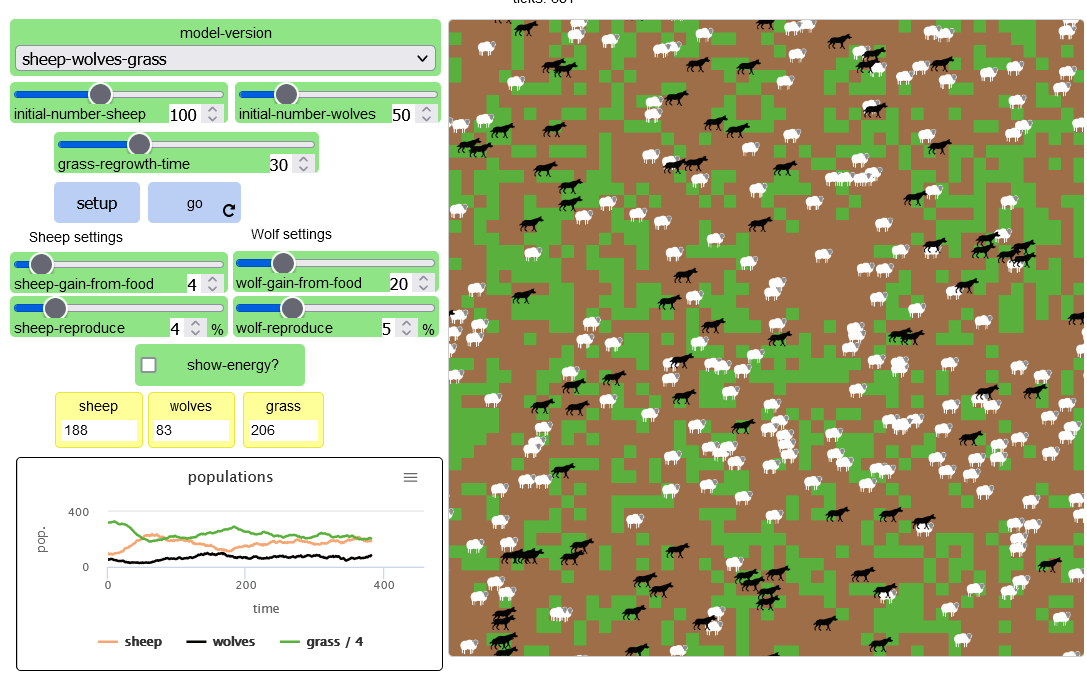
\includegraphics[scale = 0.5]{modelloNetLogo.png}
    \label{fig:ModelloNetlogo}
    \caption{La figura mostra il modello "Wolf Sheep predation" della libreria Netlogo}
\end{figure}

Oltre alle varianti appena descritte, in letteratura esistono svariati modelli di simulazione di un ecosistema naturale composto da prede e predatori realizzati in Netlogo. Gran parte di essi non si differenziano molto dai modelli standard della libreria di Netlogo. In questa sezione viene presentato quello proposto dai due ricercatori Wilensky e Rand\cite{WilenskyRand} le cui principali caratteristiche sono le seguenti: 

\begin{itemize}
    \item \emph{Tipi di agenti}: pecore, lupi, erba;
    \item \emph{Proprietà degli agenti}: energia, posizione, direzione (solo per le pecore e i lupi), quantità di erba (solo per l'erba);
    \item \emph{Comportamento degli agenti}: movimento, morte, riproduzione (solo per lupi e pecore), mangia-pecora (solo per i lupi), mangia-erba (solo per le pecore), ricrescita (solo per l'erba);
    \item \emph{Parametri}: Numero di pecore, numero di lupi, costo del movimento, energia acquisita dal cibarsi dell'erba, energia acquisita dal cibarsi delle pecore, tasso di ricrescita dell'erba.
    \item \emph{Andamento nel tempo}: Le pecore e i lupi si muovono $\rightarrow$ le pecore e i lupi muoiono $\rightarrow$ Le pecore e i lupi mangiano $\rightarrow$ Le pecore e i lupi si riproducono $\rightarrow$ l'erba ricresce
    \item \emph{Misure mostrate nei grafici}: Popolazione delle pecore in funzione del tempo, popolazione dei lupi in funzione del tempo e quantità di erba presente nel sistema sempre in funzione del tempo. 
\end{itemize}

Quest'ultimo modello appena descritto risulta essere stabile, ma, come descritto nella sezione successiva risulta essere troppo semplificato rispetto al contesto reale che intende simulare. 

\subsection{I limiti dei modelli presenti in letteratura}
I modelli descritti nelle sezioni precedenti sono certamente validi, tuttavia risultano essere troppo semplificati rispetto al fenomeno reale che intendono simulare. 
In particolare, i limiti di questi modelli sono riassumibili nei seguenti punti:
\begin{itemize}
    \item Tutti i modelli presentati in questa sezione semplificano in modo estremo la modellazione dei fenomeni di accoppiamento e di riproduzione sia delle prede che dei predatori. Infatti, nessuno dei tre modelli simula l'accoppiamento degli individui delle due specie di animali. La riproduzione in tutti e tre i casi è modellata in modo tale che ogni individuo in ogni istante di tempo abbia la possibilità di dare vita ad un cucciolo con una probabilità prefissata. Ovviamente questa è una semplificazione estrema rispetto a ciò che accade nella realtà. Infatti in un contesto reale, come ampiamente descritto nelle sezioni \ref{coniglio} e \ref{volpe} dedicate alla discussione dei caratteri delle specie coinvolte nella simulazione di questo progetto, gli animali quando sentono la necessità di riprodursi, cercano un partner ideale (ovviamente di sesso opposto) col quale accoppiarsi. Solo dopo il processo di accoppiamento può avere luogo la riproduzione. 
    \item Una seconda importante limitazione di questi modelli riguarda il fatto che qualunque tipo di animale non necessità solo di cibo per poter sopravvivere. Tutti gli animali infatti, hanno la necessità di dissetarsi tramite l'acqua che può essere localizzata in un fiume, in una pozzanghera, in un lago ecc. Nessuno dei tre modelli precedentemente presentati modella questa necessità. 
    \item Tutti e tre i modelli non considerano il concetto di percezione degli animali. Come è noto e come descritto nelle sezioni precedenti, le volpi e i conigli in particolare, ma questo vale anche per i lupi e le pecore e più in generale per qualunque tipo di animale, ogni individuo ha una certa percezione che deriva da quanto i suoi sensi (sopratutto udito, vista e olfatto) risultano essere acuti. Nessuno dei tre modelli considera questo aspetto. I modelli infatti prevedono che quando un predatore si trova sulla stessa cella della preda, esso se ne ciba uccidendola. Anche questa è una semplificazione eccessiva della realtà: i predatori spesso attuano delle strategie di caccia, sfruttando i propri sensi. Questo significa che i predatori in un contesto reale non si muovono casualmente e quando si trovano esattamente a ridosso di una preda la cacciano, bensì tendono a seguire le tracce lasciate dalle prede, a valutare la loro presenza grazie ai loro sensi e a inseguirle nel caso ne rilevino la presenza nelle vicinanze. Oltre a ciò analogamente, le prede sfruttano i propri sensi per valutare la presenza di predatori nelle vicinanze e scappare nel caso in cui ne avvertano la presenza nelle prossimità.
    \item Un'ulteriore semplificazione della realtà adottata da questi modelli risiede nel fatto che le prede possono morire per sole due cause. Esse riguardano il caso in cui esse vengano predate dai predatori e il caso in cui muoiano di fame a causa della scarsità di cibo. Invece i predatori possono morire di fame e quindi a causa della scarsità di prede a disposizione. In realtà queste non sono le uniche cause di morte. Le prede e i predatori, oltre a poter incorrere in malattie che nei casi più gravi possono portare fino al decesso, possono morire di sete (come già accennato precedentemente), oppure possono morire di vecchiaia, quando raggiunta una certa età hanno una maggior probabilità di ammalarsi. 
    \item Ulteriore semplificazione adottata dai tre modelli riguarda il fatto che in natura l'alternarsi delle quattro stagioni può portare ad effetti molto importanti nel contesto dell'ecosistema naturale simulato. La crescita dell'erba non segue un andamento costante nel tempo. In primavera e in autunno, quando le piogge sono più frequenti, essa tenderà a proliferare nell'ambiente viceversa, d'estate quando le piogge sono più rare, l'erba tende a scarseggiare. Le stesse considerazioni valgono per le masse d'acqua. Tutto ciò ha un effetto piuttosto rilevante sull'evoluzione dell'ecosistema naturale che si intende simulare. 
    \item Ogni generazione di essere vivente trasmette da una generazione alla successiva i caratteri genetici originati dall'assetto genetico.  Questo ricade sotto il nome di ereditarietà genetica. Questo aspetto non è stato in alcun modo considerato dai modelli di simulazione presentati. 
\end{itemize}


\section{Obiettivo del progetto}
L'obiettivo del progetto è stato quello di realizzare un modello di simulazione multi-agente di un ecosistema naturale. Come visto nella sezione precedente, i modelli di questo tipo presenti in letteratura sono piuttosto limitati in quanto semplificano eccessivamente la realtà che intendono simulare. L'obiettivo quindi è stato quello di eliminare le limitazioni descritte nella sezione precedente, realizzando un modello il cui ambiente fosse abitato da un gruppo di prede (i conigli) e un gruppo di predatori (le volpi). Dopo il processo di calibrazione dei parametri del modello si è optato per lo sviluppo di di tre versioni dello stesso. La prima versione, la più semplice, ha portato a risultati non del tutto soddisfacenti, per questo motivo si è deciso di affinare il modello facendo sì che un certo numero di animali (sia prede che predatori) venissero reintrodotti nell'ambiente con una certa frequenza. I risultati ottenuti con questa seconda versione sono decisamente migliori e il modello notevolmente più realistico. Infine, si è deciso di estendere ulteriormente il modello, introducendo la simulazione dell'evoluzione genetica degli animali che popolano l'ambiente. L'obiettivo è stato quello di valutare tramite simulazione come l'evoluzione genetica permetta sia ai conigli che alle volpi di adattarsi alle condizioni ambientali. Per ciascuna delle tre varianti sono stati analizzati i risultati e sono stati confrontati con quelli delle altre versioni. 

\section{Descrizione del modello}
Come già detto precedentemente, il modello sviluppato è un sistema multi-agente, composto da quattro tipologie di agenti: i Conigli (ovvero le prede), le Volpi (ovvero i predatori), l'Acqua (ovvero le pozzanghere d'acqua attraverso le quali le prede e i predatori si dissetano) e le Carote (ovvero il cibo con cui i conigli si sfamano). In questa sezione vengono illustrati l'ambiente e le quattro tipologie di agenti, oltre alla loro implementazione e i parametri del modello, divisi in base all'agente a cui fanno riferimento. Inoltre, per ognuno di essi, viene illustrato il valore finale scelto in seguito alla fase di tuning dei parametri, con la quale si è cercato di rendere il modello conforme rispetto al fenomeno reale che si intende simulare. 
\subsection{Ambiente}
L'ambiente è modellato in modo tale che fosse \textbf{continuo} e non discreto. Nella realtà il mondo è ovviamente continuo, però spesso quando si sviluppa un modello di simulazione per eseguire una semplificazione lo si discretizza generalmente per mezzo di una griglia. Nel caso specifico si è scelto di realizzare l'ambiente in modo continuo per due motivi fondamentali. Il primo riguarda il fatto che, come già detto, l'ambiente in un contesto reale non è discreto ma è continuo. La seconda motivazione è di carattere operativo: lo strumento di simulazione che è stato adottato rende possibile la gestione di un ambiente continuo in modo piuttosto semplice senza introdurre troppe complicazioni e senza aumentare eccessivamente la complessità computazionale del progetto. 

L'ambiente oltre ad essere continuo risulta essere (parzialmente) \textbf{inaccessibile}. Questo significa che ogni agente non può, in ogni istante di tempo, ottenere informazioni complete, precise e aggiornate relative allo stato dell'ambiente stesso. Infatti ogni volpe è in grado di conoscere esclusivamente le informazioni che la sua percezione le permette di ottenere. Questo significa che una volpe può sapere se c'è un coniglio, uno specchio d'acqua oppure un'altra volpe con cui accoppiarsi nelle vicinanze, ma non può conoscere (e non è nemmeno necessario) il fatto che nella posizione diametralmente opposta alla sua si trova un altro individuo della sua specie. 

L'ambiente è, inoltre, \textbf{statico}: nella finestra temporale nella quale ogni agente compie la decisione relativa al comportamento che deve tenere l'ambiente non evolve. In altre parole, questo significa che non esistono fattori esterni che influenzano e modificano l'ambiente mentre ogni agente valuta l'opportuna azione da compiere. 

L'ambiente è \textbf{deterministico}, ovvero ogni qualvolta un agente compie un'azione (per esempio una volpe decide di spostarsi verso una determinata posizione) è possibile considerare come certo l'avvenimento di tale azione. Questo però non è necessariamente vero per ciascuna azione, infatti alcune di esse risultano essere gestite tramite un processo regolato in modo stocastico. Per questo motivo le azioni così gestite, posso avvenire con un certo livello di probabilità.

Ulteriore caratteristica dell'ambiente è che esso risulta essere \textbf{episodico}. Episodico significa che ad ogni step temporale il comportamento di ogni agente è determinato considerando esclusivamente lo stato attuale del sistema. Gli agenti non sono dotati di memoria e non  mantengono traccia delle azioni precedenti. 

\subsubsection{Implementazione}
\begin{figure}[h!]
     \centering
     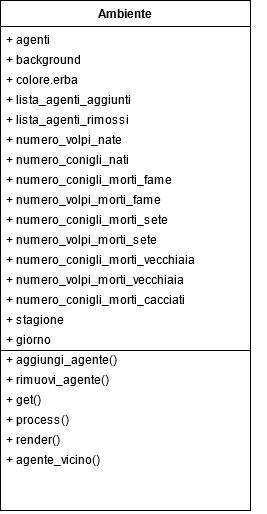
\includegraphics[scale = 0.7]{Ambiente.png}
     \caption{Diagramma della classe Ambiente}
     \label{fig:ambienteUML}
\end{figure}

L'ambiente è stato implementato attraverso un'apposita classe, le cui specifiche sono mostrate in figura \ref{fig:ambienteUML}. Gli attributi di questa classe includono la lista di agenti presenti nell'ambiente, la lista di agenti rimossi dall'ambiente dopo la loro morte, la lista di agenti aggiunti in seguito alla loro nascita, una variabile di tipo stringa denominata \emph{stagione} che indica in quale stagione si trova attualmente la simulazione, una variabile di tipo floating point denominata \emph{giorno} che permette di tenere traccia del passare del tempo durante la simulazione, una variabile denominata \emph{background} utile in fase di render dell'ambiente, una tupla denominata \emph{colore\_erba} che permette di specificare il colore con cui l'ambiente deve essere colorato in ciascuna stagione e infine, una serie di variabili intere che permettono di raccogliere i dati della simulazione in corso.

L'ambiente può eseguire le seguenti operazioni: aggiungere un agente quando esso nasce, rimuovere un'agente quando muore, restituire l'oggetto che rappresenta uno specifico agente dato il suo identificativo, eseguire il render dell'ambiente, portare avanti la simulazione in ogni istante temporale (metodo process()) e ricercare l'agente che si trova più vicino ad un altro agente passato come parametro al metodo \emph{agente\_vicino}. 
Più nello specifico, il metodo \emph{process} si occupa di mettere in atto il comportamento di ogni agente in ciascun istante temporale, di aggiungere alla simulazione gli agenti contenuti nella lista denominata \emph{lista\_agenti\_aggiunti}, di rimuovere dalla simulazione gli agenti contenuti nella lista chiamata \emph{lista\_agenti\_rimossi} e infine, di pulire le due liste. Il metodo \emph{agente\_vicino} invece, viene richiamato dagli agenti di tipo Volpe o Coniglio nel momento in cui essi devono cercare una preda da cacciare oppure un compagno con cui accoppiarsi. Il metodo prende in input le coordinate attuali dell'agente, il raggio in cui cercare (ovvero la loro percezione) e il tipo di agente da cercare. Il metodo quindi restituisce l'oggetto che fa riferimento all'agente più vicino del tipo specificato se ne è presente uno nel raggio specificato, altrimenti non restituisce nulla.    
\paragraph{Parametri}
I parametri relativi all'ambiente sono i seguenti: 
\begin{itemize}
    \item \textbf{Dimensione dell'ambiente}. Questo parametro indica la dimensione in altezza e in lunghezza espressa in pixel della finestra nel quale viene eseguito il render grafico dell'ambiente. In seguito a diverse prove, si è constatato che la dimensione dell'ambiente in rapporto al numero di agenti che lo popolano non deve essere troppo elevata. La ragione di questo è relativa al fatto che se l'ambiente fosse troppo grande, allora gli agenti si disperderebbero al suo interno. Ciononostante è altresì essenziale che la dimensione dell'ambiente non sia eccessivamente ridotta in proporzione al numero di agenti al suo interno e alla loro velocità di movimento. 
    \item \textbf{Probabilità pioggia} in primavera, estate, autunno e inverno. Questo parametro indica per ciascuna delle quattro stagioni con quale probabilità in ogni istante di tempo pioverà.
    \item \textbf{Quantità nuove pozzanghere} in primavera, estate, autunno e inverno. Indica per ogni stagione, in caso di pioggia quante pozzanghere verranno aggiunte all'ambiente. 
    \item \textbf{Probabilità aggiunta carote} in primavera, estate, autunno e inverno. Indica, per ogni stagione, la probabilità che in ogni istante di tempo venga aggiunta una carota in una posizione casuale nell'ambiente. 
    \item \textbf{Numero iniziale di agenti}. Indica il numero di agenti di tipo Coniglio, di tipo Volpe, di tipo Acqua e di tipo Carota inseriti inizialmente nel modello. 
    \item \textbf{Durata stagioni}. Indica la durata, espressa in istanti temporali, di ognuna delle quattro stagioni. 
    \item \textbf{Entità ridimensionamento pozzanghere}. Questo parametro indica di quante unità ogni istante temporale d'estate le pozzanghere vengono ridimensionate a causa del caldo che fa evaporare l'acqua. 
\end{itemize}
\vspace{2pt}
\paragraph{Tuning dei parametri}
\label{sec:tuningAmbiente}
Di seguito viene esposto il valore con cui sono stati settati i parametri descritti nel paragrafo precedente.
\begin{table}[h!]
\centering
\begin{tabular}{@{}lll@{}}
\toprule
                         & Larghezza (pixel) & Altezza (pixel) \\ \midrule
Dimensione dell'ambiente & 1200      & 800      
\end{tabular}
\end{table}

\vspace{5pt}

\begin{table}[h!]
\centering
\begin{tabular}{l|cccc}
                          & Volpe & Coniglio & Acqua & Carota \\ \hline
Numero iniziale di agenti & 25    & 75       & 200   & 250   
\end{tabular}
\end{table}

\begin{table}[h!]
\centering
\begin{tabular}{p{0.4\textwidth}|cccc}
& \multicolumn{4}{c}{Stagione} \\   
\hline
Parametro & \multicolumn{1}{l}{Primavera} & \multicolumn {1}{l}{Estate} & \multicolumn{1}{l}{Autunno} & \multicolumn{1}{l}{Inverno} \\
\hline
Probabilità pioggia  & 0.285\%  & 0.1\%  & 0.5\% & 0.4\% \\
Quantità nuove pozzanghere & rand(0,10) & rand(0,50) & rand(0,10) & rand(0,10) \\
Probabilità aggiunta carote & 33\% & 20\% & 10\% & 20\% \\
Durata stagioni & 500 & 500 & 500 & 500 \\
Probabilità ridimensionamento pozzanghere & -  & 1  & - & -                          
\end{tabular}
\end{table}





%L'ambiente è stato implementato in modo tale che dovesse eseguire le seguenti operazioni: 
%\begin{itemize}
    %\item mantenere traccia degli agenti che operano in esso;
    %\item gestire il render della superficie dell'ambiente stesso. Il colore della superficie cambia in base alla stagione: in primavera ha è di un verde intenso in estate è arancione, in autunno è verde meno intenso e infine di inverno è bianco;
    %\item gestire la nascita e la morte degli agenti. L'ambiente mantiene traccia di tutti gli agenti che muoiono e nascono e si occupa della rimozione di quelli morti e dell'aggiunta di quelli nati in ogni istante temporale
    %\item dato un agente e un range, valutare quale è (se esiste) l'agente più vicino ad esso all'interno del range indicato;
    %\item mantenere le informazioni relative agli agenti, quali il numero di volpi morte di sete, il numero di volpi morte di fame e così via;
    %\item eseguire il render di tutti gli agenti del sistema e dell'ambiente stesso. 
%\end{itemize}

\subsection{Agenti}
Il modello sviluppato è composto da un totale di quattro tipi di agenti: volpi, conigli, carote e pozzanghere d'acqua. Di seguito vengono descritte le caratteristiche generali i parametri e il comportamento di ognuno di essi. 

\subsubsection{Acqua}
Questo agente è il più semplice insieme all'agente \emph{Carota} e rappresenta gli specchi d'acqua (pozzanghere) attraverso i quali le volpi e i conigli hanno la possibilità di soddisfare il proprio bisogno di dissetarsi. Sono distribuite in modo casuale nell'ambiente e possono essere sfruttate dalle prede e dai predatori fino ad un massimo di tre volte prima di scomparire. Appaiono nell'ambiente con frequenza differente nelle quattro stagioni, come mostrato nella sezione \ref{sec:tuningAmbiente}.  

\subsubsection{Implementazione}
\begin{figure}[h!]
     \centering
     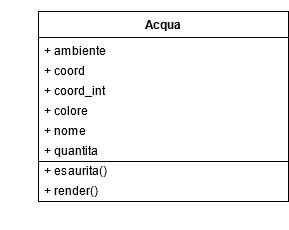
\includegraphics[scale = 0.7]{Acqua.png}
     \label{fig:acquaUML}
     \caption{Diagramma della classe Acqua}
\end{figure}

Gli attributi della classe Acqua sono i seguenti:
\begin{itemize}
    \item \textbf{ambiente}: è un riferimento all'oggetto Ambiente. 
    \item \textbf{coord}. Si tratta di un vettore in due dimensioni che rappresenta le coordinate dove si trova la rispettiva pozzanghera d'acqua nell'ambiente. 
    \item \textbf{coord\_int}. Analogo a coord, solo che \emph{coord\_int} è espresso tramite numeri interi e non decimali. 
    \item \textbf{colore}. Indica il colore con cui dovrà essere eseguito il render degli agenti di questo tipo.
    \item \textbf{nome}. Si tratta di una stringa con la quale vengono identificati gli agenti appartenenti a questa categoria. 
    \item \textbf{quantità}. Indica la dimensione della pozzanghera. Può assumere valori interi compresi tra 0 e 3. 3 significa che la pozzanghera può essere sfruttata ancora da 3 conigli e/o volpi prima di essere eliminata dall'ambiente, 0 significa che la pozzanghera deve essere rimossa dall'ambiente, in quanto è stata già sfruttata 3 volte dalle volpi e dai conigli e quindi risulta essere esaurita. 
\end{itemize}

I metodi \emph{esaurita} e \emph{render} permettono rispettivamente di chiedere all'ambiente l'eliminazione dell'agente e di eseguire il render grafico degli agenti che rappresentano le pozzanghere nell'ambiente. 



\subsubsection{Carota}
Questa tipologia di agente rappresenta ciò di cui i conigli si cibano per potersi sostentare. Anche le carote, così come le pozzanghere d'acqua, sono distribuite in modo casuale nell'ambiente. Le carote però, a differenza degli specchi d'acqua, una volta che sono state mangiate dai conigli scompaiono dall'ambiente e non possono essere ulteriormente mangiate da altri conigli. Così come per l'acqua, anche le carote vengono distribuite sul territorio con un frequenza che varia in base alla stagione, come illustrato nella sezione \ref{sec:tuningAmbiente}. 

\subsubsection{Implementazione}

\begin{figure}[h!]
     \centering
     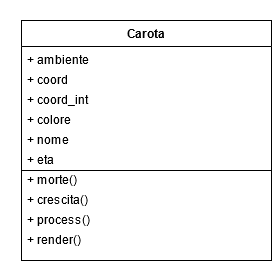
\includegraphics[scale = 0.7]{Carota.png}
     \label{fig:carotaUML}
     \caption{Diagramma della classe Carota}
\end{figure}
 Gli attributi degli agenti di tipo Carota sono i seguenti: 
\begin{itemize}
    \item \textbf{ambiente}. Si tratta di un riferimento all'oggetto della classe Ambiente. 
    \item \textbf{coord}. Si tratta di un vettore in due dimensioni, che rappresenta le coordinate che identificano la locazione all'interno dell'ambiente della carota. 
    \item \textbf{coord\_int}. Analogo a coord, la differenza risiede nel fatto che \emph{coord\_int} è espresso tramite numeri interi e non decimali. 
    \item \textbf{colore}. Indica il colore con cui dovrà essere eseguito il render degli agenti di questo tipo.
    \item \textbf{nome}. Si tratta di una stringa, utile per identificare gli agenti che appartengono a questa categoria. 
    \item \textbf{eta}. Indica da quanto tempo la carota è presente nell'ambiente. Una volta che la carota è presente nell'ambiente per troppo tempo verrà rimossa, in quanto marcita. 
\end{itemize}

I metodi della classe Carota sono i seguenti:
\begin{itemize}
    \item \textbf{morte}. Questo metodo viene invocato ogni qualvolta una carota viene mangiata da un coniglio, oppure marcisce. Esso chiede all'ambiente di rimuovere il rispettivo agente. 
    \item \textbf{crescita}. Questo metodo permette con una probabilità pari a 0.05\% di far nascere una nuova carota nelle vicinanze dell'agente che lo richiama (in un raggio di 50 pixel).
    \item \textbf{process}. Questo metodo, richiamato in ogni istante temporale della simulazione, esegue le seguenti operazioni: 
    \begin{itemize}
        \item richiama il metodo \emph{crescita}, descritto nel punto precedente;
        \item incrementa l'attributo \emph{eta} dell'agente di 0.03;
        \item nel caso in cui l'età della carota dovesse aver raggiunto un valore superiore a 2.5 cambia il colore con cui essa viene mostrata in modo da evidenziare che essa sta per marcire e quindi per sta per essere rimossa dalla simulazione;
        \item nel caso in cui la carota dovesse avere un'età superiore a 3, chiede all'ambiente di rimuovere l'agente. 
    \end{itemize}
    \item \textbf{render}. Questo metodo permette di eseguire il render grafico dell'agente nella corretta posizione dell'ambiente. 
\end{itemize}
\subsubsection{Coniglio e Volpe}
Gli agenti di tipo \emph{Coniglio} rappresentano le prede dell'ecosistema naturale che si intende simulare, mentre gli agenti di tipo \emph{Volpe} rappresentano i predatori. I due agenti sono stati implementati tramite le classi Coniglio e Volpe, che, come si può vedere dalla figura \ref{fig:ConiglioVolpeUML}, condividono la stessa struttura. 

\subsubsection{Implementazione}
\begin{figure}[h!]
     \centering
     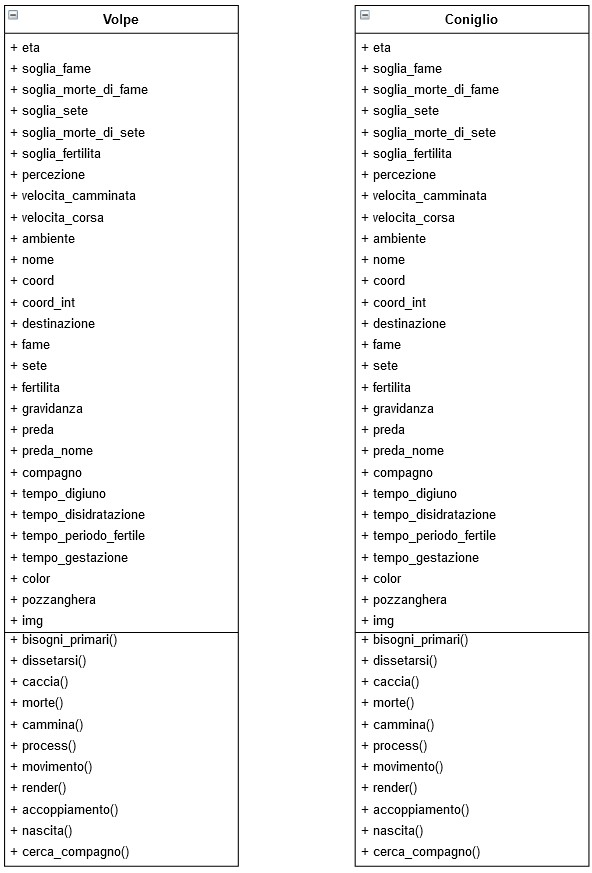
\includegraphics[scale = 0.7]{Animale.png}
     \caption{Diagrammi delle classi Coniglio e Volpe}
     \label{fig:ConiglioVolpeUML}
\end{figure}
Gli attributi relativi agli agenti Coniglio e Volpe sono i seguenti: 
\begin{itemize}
    \item \textbf{età}. Indica l'età dell'agente. In ogni istante temporale questo valore viene incrementato di 0.03. Conigli e Volpi di età superiore a 4 o inferiore a 0.5 hanno percezione e velocità di corsa dimezzata rispetto a quella degli animali adulti. Inoltre Conigli e Volpi con età inferiore a 0.5 non possono accoppiarsi. 
    \item \textbf{percezione}. Questo attributo indica il raggio di percezione dell'agente. Un valore alto indica che l'agente può vedere e sentire predatori da grande distanza, viceversa un valore basso sta a significare che l'agente può vedere e percepire la presenza di altri agenti (quali pozze d'acqua, carote o volpi) solo nel momento in cui si trovano a distanze ridotte rispetto al punto in cui esso si trova. 
    \item \textbf{ambiente}. Si tratta di un riferimento all'oggetto della classe Ambiente, precedentemente descritta. 
    \item \textbf{nome}. Si tratta di una stringa che indica il tipo di agente. 
    \item \textbf{coord}.Esso è un vettore in due dimensioni che identifica la posizione dell'agente in ogni istante temporale. 
    \item \textbf{coord\_int}. Indica la posizione attuale dell'agente tramite coordinate intere.
    \item \textbf{destinazione}. Indica la destinazione dell'agente. Inizialmente ogni coniglio e ogni volpe hanno una destinazione che viene fissata in modo casuale. Successivamente, nel momento in cui l'agente percepisce la necessità di accoppiarsi e trova un compagno nelle vicinanze con cui accoppiarsi, questo parametro viene impostato in modo tale che la destinazione sia pari alle coordinate della posizione dell'altro agente. Analogamente, quando un animale ha necessità di dissetarsi e vede una pozzanghera nell'intorno della propria percezione, allora la destinazione viene impostata in modo tale che sia pari alle coordinate della pozzanghera. Infine, avviene lo stesso anche quando l'agente ha necessità di cibarsi e nota la presenza di una preda (che sarà un coniglio nel caso delle volpi e una carota nel caso dei conigli) sempre nell'intorno della propria percezione. 
    Invece nel caso in cui l'agente non ha né la necessità di bere, né quella di mangiare né quella di accoppiarsi, allora la sua destinazione verrà impostata in modo casuale in modo tale che esso si muova liberamente nell'ambiente. 
    \item \textbf{fame}. Si tratta di un valore booleano che indica se l'agente ha necessità di sfamarsi o meno. Inizialmente il valore è pari a False e nel momento in cui il numero di step temporali passati senza che abbia mangiato diventa superiore al parametro \emph{soglia\_fame} il suo valore viene impostato a True. 
    \item \textbf{sete}. Anche in questo caso si tratta di un valore booleano. Esso indica se l'agente necessita o meno di bere. Anche in questo caso, esso inizialmente è impostato a False e appena il tempo passato dall'agente senza bere diventa superiore al valore del parametro \emph{soglia\_disidratazione} il suo valore viene impostato a True. 
    \item \textbf{fertilità}. Si tratta di un valore booleano che indica se l'agente sente il bisogno e ha la necessità di riprodursi oppure no. 
    \item \textbf{gravidanza}. Anch'esso è un parametro di tipo booleano e indica se l'agente risulta essere in attesa di una cucciolata o meno. Nel primo caso, dopo un certo periodo di gestazione, esso darà alla luce i cuccioli. 
    \item \textbf{preda}. Fa riferimento ad un agente di tipo \emph{Carota} nel caso dei conigli e un agente di tipo \emph{Coniglio} nel caso delle volpi e rappresenta la preda identificata dall'agente per potersi cibare. 
    \item \textbf{preda\_nome}. Si tratta di una stringa che identifica il tipo di preda: coniglio per le volpi e carota per i conigli. 
    \item \textbf{compagno}. Esso rappresenta un agente con cui l'animale ha intenzione di accoppiarsi. 
    \item \textbf{tempo\_digiuno}. Si tratta di un parametro che indica il tempo passato dall'ultimo istante in cui l'agente si è cibato.
    \item \textbf{tempo\_disidratazione}. Indica quanti istanti temporali sono trascorsi dall'ultima volta che l'agente si è abbeverato in una pozzanghera. 
    \item \textbf{tempo\_periodo\_fertile}. Indica quanto tempo è passato dall'ultimo accoppiamento dell'animale. 
    \item \textbf{tempo\_gestazione}. Indica il tempo che deve passare dal momento in cui l'agente si è accoppiato con un altro agente e il momento in cui esso da alla luce i cuccioli. 
    \item \textbf{pozzanghera}. Indica un agente di tipo Acqua che l'agente ha avvistato per potersi dissetare.
    \item \textbf{color}. Indica il colore con cui eseguire il render dell'agente. Questo attributo viene considerato solo nel momento in cui la simulazione viene lanciata con l'attributo GRAFICA impostato a False. Vedere la sezione \ref{sec:codice} per maggiori dettagli in tal senso. 
    \item \textbf{img}. Indica l'immagine con cui eseguire il render dell'agente. Questo attributo viene considerato solo per le simulazioni lanciate con l'attributo GRAFICA settato a True. Fare riferimento anche in questo caso alla sezione \ref{sec:codice} per maggiori dettagli in tal senso. 
    \item \textbf{soglia\_fame}. Si tratta di una soglia, superata la quale l'agente inizia ad avere necessità di cibarsi (di carote nel caso dei conigli e di conigli nel caso delle volpi).
    \item \textbf{soglia\_morte\_di\_fame}. Si tratta della soglia superata la quale l'agente morirà di fame. In altre parole, significa che se un coniglio o una volpe rimangono senza mangiare per un numero di istanti temporali superiore a tale soglia, allora esso morirà di fame.
    \item \textbf{soglia\_sete}. Indica la soglia oltre la quale l'agente inizia a percepire la necessita di dissetarsi. 
    \item \textbf{soglia\_morte\_di\_sete}. Così come per la fame, anche questa soglia è rappresentativa del fatto che se un agente passa un numero di time step senza bere superiore rispetto a questa soglia,  esso morirà di sete e verrà rimosso dall'ambiente. 
    \item \textbf{soglia\_fertilità}. Indica la soglia oltre la quale l'agente sentirà la necessità di accoppiarsi. Anche in questo caso, una volta passati un numero di time step senza che il coniglio si sia accoppiato, superiore a questa soglia, l'agente inizierà a sentire la necessita di accoppiarsi e quindi di riprodursi.
    \item \textbf{velocità\_camminata}. Questo parametro indica la velocità con cui si sposta l'agente in condizioni normali, ovvero quando non è inseguito da un predatore, non è alla ricerca di un compagno e non è alla ricerca di cibo con cui sfamarsi.  
    \item \textbf{velocità\_corsa}. Questo parametro invece, indica la velocità con cui l'agente si muove nelle seguenti condizioni: l'agente ha trovato un compagno con cui accoppiarsi, l'agente ha trovato una pozzanghera da cui abbeverarsi oppure l'animale ha trovato una preda di cui cibarsi nell'area circolare avente come centro la propria posizione e come raggio il valore della sua percezione.
    \item \textbf{eta\_morte\_vecchiaia}. Questo parametro indica a quale età le volpi e i conigli muoiono di vecchiaia.
\end{itemize}

\paragraph{comportamento degli agenti Volpe e Coniglio}

Il metodo \emph{bisogni\_primari}, come si può intuire dal nome stesso, si occupa della gestione dei bisogni primari degli agenti di tipo Volpe e di tipo Coniglio. Entrambe queste categorie di agenti hanno tre necessità: cacciare (le volpi cacciano i conigli e i conigli si cibano delle carote) per non morire di fame, dissetarsi per non morire di sete e infine, accoppiarsi per potersi riprodurre. 

La gestione dei bisogni primari avviene come mostrato in figura \ref{fig:diagrammaComportamentale}. 
\begin{figure}
     \centering
     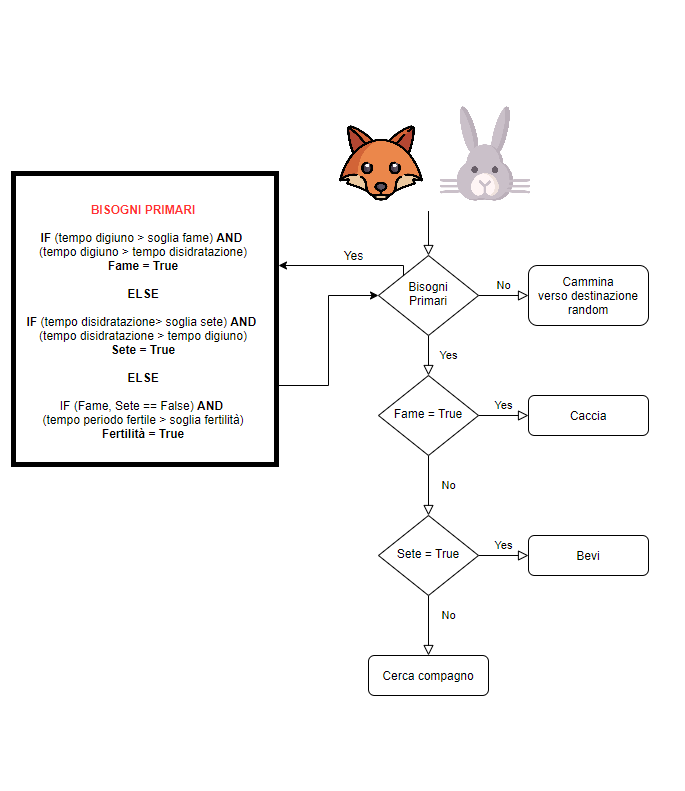
\includegraphics[scale = 0.7]{diagramma_comportamentale.png}
     \label{fig:diagrammaComportamentale}
     \caption{Il diagramma in figura mostra il comportamento degli agenti di tipo Volpe e di tipo Coniglio ad ogni iterazione.}
\end{figure}
Come si vede in tale immagine, per prima cosa si valuta se l'agente è morto di fame o di sete e nel caso viene richiamato il metodo \emph{morte} descritto in seguito.  Successivamente si valuta se l'agente ha una delle tre necessità. Per far ciò per prima cosa viene considerato il tempo passato dall'ultima volta che l'animale si è cibato (valore memorizzato nella variabile \emph{tempo\_digiuno}) e il valore del tempo trascorso dall'ultimo istante in cui l'animale si è dissetato (memorizzato nella variabile \emph{tempo\_disidratazione}). Se il primo dei due valori è maggiore del valore di \emph{soglia\_fame} e del valore della variabile \emph{tempo\_disidratazione}, allora il valore della variabile booleana \emph{fame} viene settato a True. In seguito, si valuta se il tempo trascorso dall'ultima volta che l'animale si è dissetato è maggiore del valore di \emph{soglia\_sete} e del valore che indica il tempo trascorso dall'ultimo momento in cui l'animale si è sfamato. In caso affermativo allora il valore della variabile booleana \emph{sete} viene settato a True. Infine, se il tempo trascorso dall'ultima volta che l'animale si è cibato è minore del valore \emph{soglia\_fame} e il tempo trascorso dall'ultima volta che l'animale si è dissetato è minore di \emph{soglia\_sete} e il tempo trascorso dall'ultima volta che l'animale si è accoppiato (memorizzato nella variabile \emph{tempo\_periodo\_fertile}) è maggiore del valore assunto dal parametro \emph{soglia\_fertilità}, allora il valore della variabile booleana \emph{fertilita} viene settato a True. 

In seguito a tali valutazioni, se nessuna delle tre variabili \emph{fame}, \emph{sete} e \emph{fertilita} ha assunto un valore pari a True, allora l'agente cammina verso una destinazione fissata in modo casuale all'interno dell'ambiente. Viceversa, se il valore della variabile \emph{fame} è diventato pari a True, allora l'agente inzia la procedura denominata \emph{Caccia}, descritta successivamente. Nel caso in cui la variabile \emph{fame} sia False e la variabile \emph{sete} sia True, allora l'agente inizia la procedura denominata \emph{Bevi}, descritta in seguito. Infine, nel caso in cui sia la variabile \emph{fame} che la variabile \emph{sete} sono pari a False e la variabile \emph{fertilita} ha assunto valore pari a True, allora l'agente inizia la procedura \emph{Cerca compagno}, descritta anch'essa successivamente in questa sezione. 

Il metodo \emph{caccia} permette di attivare la procedura denominata in modo analogo, attraverso la quale i Conigli possono cercare carote nelle vicinanze per potersi sfamare e le volpi possono cercare dei conigli nelle vicinanze in modo tale da poterli cacciare per poter soddisfare la propria necessità di cibarsi.
\begin{figure}
     \centering
     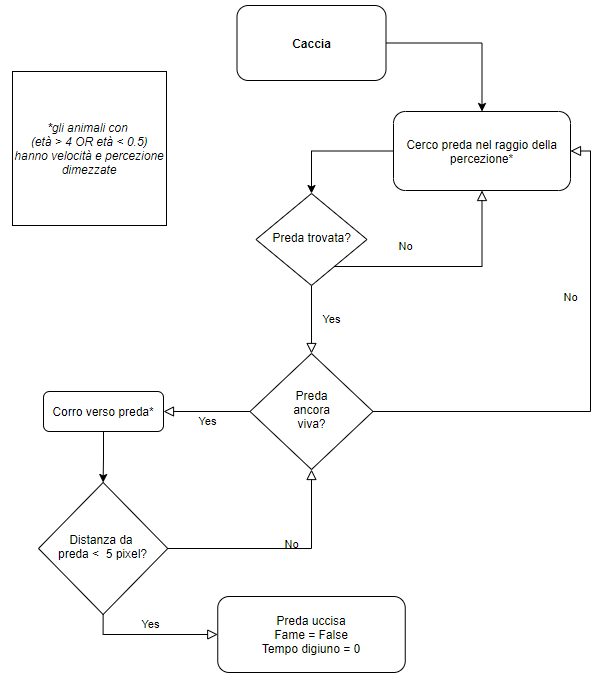
\includegraphics[scale = 0.7]{Caccia.png}
     \label{fig:diagrammaCaccia}
     \caption{Il diagramma in figura mostra come si comportano i conigli e le volpi quando hanno la necessità di cibarsi}
\end{figure}
Come visibile nella figura \ref{fig:diagrammaCaccia}, l'agente per prima cosa cerca se c'è una preda nell'area circolare avente come centro la posizione attuale dell'agente e come raggio la sua percezione. Si noti che per i cuccioli e per gli anziani (ovvero quelle volpi e quei conigli che hanno età inferiore a 0.5 o superiore a 4) la loro percezione viene dimezzata. Se l'agente non trova una preda (una carota nel caso dei conigli, un coniglio nel caso delle volpi), allora esso camminerà verso un punto posizionato in modo casuale nell'ambiente e al prossimo istante temporale la procedura verrà ripetuta dall'inizio. 
Viceversa, nel caso in cui l'agente dovesse trovare una preda nei dintorni, allora l'ambiente comunica all'agente se la preda è ancora viva oppure no. Quest'ultima valutazione si rende utile per evitare il presentarsi di alcuni conflitti che occorrerebbero nel momento in cui un agente ha trovato una preda, ma prima che esso possa raggiungerla, un altro agente se ne ciba rendendola non più disponibile per il primo agente.
Nel caso in cui la preda non dovesse essere più presente nell'ambiente, allora l'agente si muove verso una destinazione random e ripete dall'inizio la procedura. Invece, nel caso in cui la preda dovesse essere ancora viva, l'agente inizia a correre verso la preda. Si noti che la velocità di corsa dei cuccioli e degli anziani è dimezzata rispetto a quella degli agenti adulti. Nel momento in cui la preda risulterà essere ad una distanza ridotta (inferiore a 5 pixel), allora la preda verrà uccisa, il parametro \emph{fame} dell'agente viene posto a False e l'attributo \emph{tempo\_digiuno} viene settato con un valore pari a zero. Se invece la distanza dovesse essere superiore a 5 pixel, l'agente chiede nuovamente all'ambiente se la preda è ancora viva e la procedura si ripete. 

Il metodo \emph{dissetarsi} permette di dare inizio alla procedura denominata \emph{bevi}, mostrata nel diagramma visualizzato nella figura \ref{fig:diagrammaBevi}. 
\begin{figure}
     \centering
     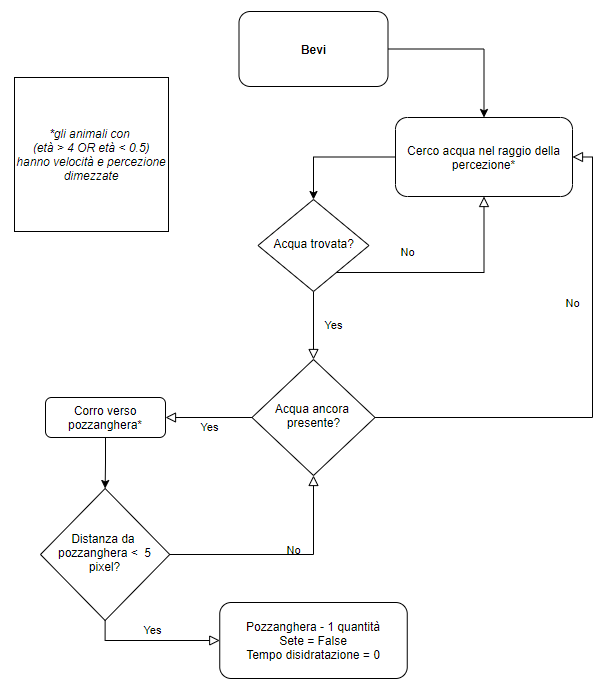
\includegraphics[scale = 0.7]{Sete.png}
     \label{fig:diagrammaBevi}
     \caption{Il diagramma in figura mostra come si comportano i conigli e le volpi quando hanno la necessità di dissetarsi}
\end{figure}
Questa procedura permette sia ai conigli che alle volpi di cercare una pozzanghera d'acqua per soddisfare la propria sete. Essa prevede in primo luogo che l'agente cerchi una pozzanghera nell'area circolare avente come centro la posizione attuale dell'agente e come raggio la percezione dell'agente stesso. Si noti che anche in questa situazione valgono le considerazioni di cui sopra: i cuccioli (età minore di 0.5) e gli anziani (età superiore a 4) hanno valori di percezione e velocità dimezzate rispetto a quelle degli adulti. Se l'ambiente comunica all'agente che non esiste una pozzanghera nei dintorni, allora l'agente si muove con destinazione casuale nell'ambiente e dal prossimo istante temporale la procedura viene riapplicata dall'inizio. Viceversa, nel caso in cui l'ambiente comunica all'agente che esiste una pozzanghera nelle vicinanze, allora l'agente inizia a correre verso la posizione della pozzanghera. In ogni istante temporale l'ambiente comunica all'agente se la pozzanghera è ancora presente nell'ambiente o meno (potrebbe accadere che altri agenti nel frattempo si sono diretti verso la stessa direzione e abbiano esaurito la pozzanghera). In caso negativo l'agente si dirige camminando verso una destinazione casuale e nel successivo istante temporale ripete la procedura dall'inizio. Se invece l'ambiente comunica all'agente che la pozzanghera non è stata esaurita da altri agenti, allora esso continua la corsa verso di essa. Questo ciclo si ripete fino a quando la distanza tra la pozzanghera e l'agente risulta essere inferiore a 5 pixel. In questa situazione l'agente si disseta, quindi il valore dell'attributo \emph{sete} diventa False, viene diminuita di una unità la dimensione della pozzanghera (che inizialmente ha una dimensione pari a 3) e l'attributo \emph{tempo\_disidratazione} dell'agente viene impostato con un valore pari a zero. 

Il metodo \emph{cerca\_compagno} permette di dare inizio alla procedura denominata in modo analogo, che permette alle volpi e ai conigli di cercare un animale della propria specie con cui accoppiarsi ed è illustrata con un diagramma visibile nella figura \ref{fig:diagrammaAccoppiamento}.
\begin{figure}
     \centering
     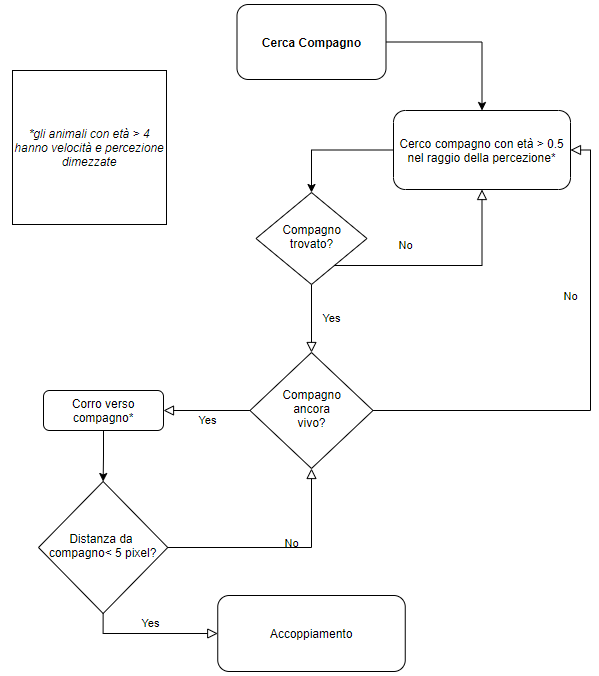
\includegraphics[scale = 0.7]{Cerca_Compagno.PNG}
     \label{fig:diagrammaAccoppiamento}
     \caption{Il diagramma in figura mostra come si comportano i conigli e le volpi quando hanno la necessità di accoppiarsi}
\end{figure}
Per prima cosa ogni agente che ha la necessità di accoppiarsi chiede all'ambiente se ci sono altri agenti dello stesso tipo e con età maggiore di 0.5 (i cuccioli non si possono accoppiare) nell'area circolare centrata nella posizione attuale dell'agente e di raggio pari alla percezione dello stesso.
In caso negativo l'agente si muove verso una direzione casuale nell'ambiente e dall'istante di tempo successivo riprende dall'inizio l'esecuzione della procedura. Viceversa, in caso affermativo l'ambiente comunica la posizione del candidato compagno più vicino. L'agente inizia a correre verso la posizione comunicatagli dall'ambiente e in ogni istante temporale chiede all'ambiente se il compagno è ancora vivo. In caso negativo esso si sposta verso una destinazione casuale per poi ripetere l'intera procedura. Se invece, l'ambiente comunica che il compagno è ancora vivo, allora l'agente continua la corsa verso di esso. Questa operazione viene continuamente ripetuta in ogni istante temporale fino a quando la distanza tra i due agenti risulta essere inferiore a 5 pixel. In questo caso l'accoppiamento vero e proprio può avere luogo, richiamando il metodo \emph{accoppiamento}. 

L'accoppiamento viene gestito in questo modo: gli attributi \emph{fertilita} dei due agenti coinvolti nell'accoppiamento vengono impostati a False, gli attributi \emph{tempo\_periodo\_fertile}, che indicano quanto tempo è passato dall'ultimo accoppiamento dell'agente, vengono posti a 0 e inoltre l'attributo \emph{gravidanza} di uno dei due agenti viene impostato a True.
Dopo di questo viene richiamato il metodo \emph{nascita} e dopo un periodo di gestazione, avviene la nascita  dei cuccioli(vedere il paragrafo \ref{sec:tuningAmbiente} per informazioni relative al numero di cuccioli che nascono ad ogni parto e ai tempi di gestazione delle due tipologie di agenti). Nelle versioni del modello che non prevedono la gestione dell'evoluzione genetica i parametri \emph{soglia\_fame}, \emph{soglia\_morte\_di\_fame}, \emph{soglia\_sete}, \emph{soglia\_morte\_di\_sete}, \emph{soglia\_fertilità}, \emph{percezione}, \emph{velocita\_camminata} e \emph{velocita\_corsa} dei cuccioli vengono impostati seguendo il seguente principio: 
\[
    y = rand(min(x_1, x_2), max(x_1, x_2))
\]
Dove $x$ è il valore ereditato dal cucciolo e $x_1$ e $x_2$ sono i rispettivi parametri dei due genitori.  Viceversa, nella versione del modello in cui è stata implementata l'evoluzione genetica,
ogni qualvolta nasce un cucciolo i parametri \emph{soglia\_fame}, \emph{soglia\_morte\_di\_fame}, \emph{soglia\_sete}, \emph{soglia\_morte\_di\_sete}, \emph{soglia\_fertilità}, \emph{percezione}, \emph{velocita\_camminata} e \emph{velocita\_corsa} dei cuccioli vengono ereditati dai genitori seguendo questo approccio:
\[
    y = rand(min(x_1, x_2), max(x_1, x_2)) + rand(-y1, y1) 
\]
Dove $y$ è il parametro ereditato dal cucciolo e $x_1, x_2$ sono i rispettivi parametri dei due genitori. Invece, $y_1$ è un offset appositamente scelto per ognuno degli otto parametri. Un valore grande implica che i cambiamenti genetici, anche nel breve periodo, siano più ampi, mentre se viene scelto un valore basso i cambiamenti genetici, almeno nel breve periodo,  risultano essere piuttosto contenuti. 
Un esempio di questo comportamento è mostrato in figura \ref{fig:EsempioEvoluzione}. 
\begin{figure}[h!]
     \centering
     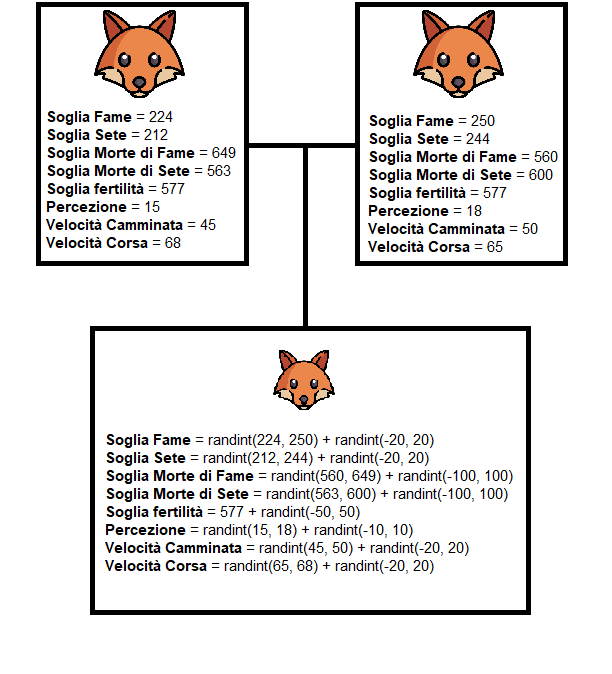
\includegraphics[scale = 0.8]{Accoppiamento_evoluzione.png}
     \label{fig:EsempioEvoluzione}
     \caption{Il diagramma in figura mostra un esempio concreto di come viene gestita l'ereditarietà dei caratteri nel modello.}
\end{figure}

Invece, il metodo \emph{morte} viene richiamato quando un animale muore di vecchiaia, muore di sete, muore di fame oppure muore cacciato da un predatore (ovviamente quest'ultimo caso è valevole solo per i conigli che vengono cacciati dalle volpi). La prima situazione si verifica quando il valore \emph{eta} dell'agente supera il valore 4.5 nel caso dei conigli e il valore 5 nel caso delle volpi. Una volpe o un coniglio, invece muore di sete quando il valore \emph{tempo\_disidratazione} diventa maggiore del parametro \emph{soglia\_morte\_di\_sete}. Analogamente, un animale muore di fame quando il valore \emph{tempo\_digiuno} diventa superiore al parametro \emph{soglia\_morte\_di\_fame}. In tutti questi casi viene richiamato il metodo \emph{morte} che si occupa di aggiungere l'agente alla lista di agenti da rimuovere. Sarà poi compito dell'ambiente occuparsi della rimozione vera e propria dell'agente dall'ambiente. 

Il metodo \emph{cammina}, con l'ausilio del metodo \emph{movimento}, permette di spostare l'agente verso la propria destinazione con velocità pari a quella indicata nel parametro \emph{velocita\_camminata}. 

Infine, il metodo \emph{process} si occupa del coordinamento di tutte le operazioni descritte fino ad ora. Esso viene richiamato in ciascun istante temporale e effettua le seguenti operazioni:
\begin{itemize}
    \item incrementare di una unità il valore delle variabili \emph{tempo\_digiuno} e \emph{tempo\_disidratazione};
    \item incrementare di 0.003 il valore dell'attributo \emph{eta} dell'agente;
    \item nel caso in cui l'età dell'agente sia maggiore di 0.5, aumentare il valore dell'attributo \emph{tempo\_periodo\_fertile} di una unità;
    \item valutare se l'agente ha raggiunto un'età tale per cui esso deve morire di vecchiaia e nel caso richiamare il metodo \emph{morte};
    \item richiamare il metodo \emph{bisogni\_primari} per la gestione delle necessità dell'agente;
    \item far muovere l'agente
\end{itemize}

In ultimo luogo, il metodo \emph{render} viene richiamato per eseguire il render grafico dell'agente all'interno dell'ambiente.

\begin{comment}
\paragraph{parametri}
I parametri del modello relativi agli agenti di tipo Coniglio e Volpe sono i seguenti: 
\begin{itemize}
    \item \textbf{soglia\_fame}. Si tratta di una soglia, superata la quale l'agente inizia ad avere necessità di cibarsi (di carote nel caso dei conigli e di conigli nel caso delle volpi).
    \item \textbf{soglia\_morte\_di\_fame}. Si tratta della soglia superata la quale l'agente morirà di fame. In altre parole, significa che se un coniglio o una volpe rimangono senza mangiare per un numero di istanti temporali superiore a tale soglia, allora esso morirà di fame.
    \item \textbf{soglia\_sete}. Indica la soglia oltre la quale l'agente inizia a percepire la necessita di dissetarsi. 
    \item \textbf{soglia\_morte\_di\_sete}. Così come per la fame, anche questa soglia è rappresentativa del fatto che se un agente passa un numero di time step senza bere superiore rispetto a questa soglia,  esso morirà di sete e verrà rimosso dall'ambiente. 
    \item \textbf{soglia\_fertilità}. Indica la soglia oltre la quale l'agente sentirà la necessità di accoppiarsi. Anche in questo caso, una volta passati un numero di time step senza che il coniglio si sia accoppiato, superiore a questa soglia, l'agente inizierà a sentire la necessita di accoppiarsi e quindi di riprodursi.
    \item \textbf{velocità\_camminata}. Questo parametro indica la velocità con cui si sposta l'agente in condizioni normali, ovvero quando non è inseguito da un predatore, non è alla ricerca di un compagno e non è alla ricerca di cibo con cui sfamarsi.  
    \item \textbf{velocità\_corsa}. Questo parametro invece, indica la velocità con cui l'agente si muove nelle seguenti condizioni: l'agente ha trovato un compagno con cui accoppiarsi, l'agente ha trovato una pozzanghera da cui abbeverarsi oppure l'animale ha trovato una carota di cui cibarsi nell'area circolare avente come centro la propria posizione e come raggio il valore della sua percezione.
    \item \textbf{eta\_morte\_vecchiaia}. Questo parametro indica a quale età le volpi e i conigli muoiono di vecchiaia.
\end{itemize}
\end{comment}
\paragraph{Tuning dei parametri}
\label{sec:tuningAnimali}
Nella tabella sottostante viene esposto il valore con cui sono stati settati i parametri descritti nel paragrafo precedente.

\begin{table}[]
\centering
\begin{tabular}{l|cc}
\multicolumn{1}{c|}{Parametro} & Volpe          & Coniglio      \\ \hline
soglia\_fame                   & rand(200; 250) & rand(200;250) \\
soglia\_morte\_di\_fame        & rand(550;650)  & rand(500;600) \\
soglia\_sete                   & rand(200;250)  & rand(200;250) \\
soglia\_morte\_di\_sete        & rand(550;650)  & rand(500;600) \\
soglia\_fertilita              & rand(500;600)  & rand(250;300) \\
percezione                     & rand(15;20)    & rand(15;20)   \\
velocita\_camminata            & rand(40;60)    & rand(40;60)   \\
velocita\_corsa                & rand(65;75)    & rand(65;75)   \\
eta\_morte\_vecchiaia          & 5              & 4.5
\end{tabular}
\end{table}




\begin{comment}
\subsection{Implementazione del comportamento degli agenti}
Il ciclo di vita degli agenti di tipo Acqua è estremamente semplice. All'inizio della simulazione un certo numero di agenti di questo tipo viene disposto in modo casuale nell'ambiente. Ognuno di essi ha un parametro chiamato quantità che indica quante volte i conigli e le volpi potranno abbeverarsi dalla stessa pozzanghera prima che essa venga rimossa dall'ambiente. Questo valore è identico per ogni agente ed è stato fissato a 3. Con il passare del tempo, nuove pozzanghere vengono disposte nell'ambiente, in modo più o meno frequente nelle varie stagioni. La frequenza di apparizione di nuove pozzanghere è stata gestita in modo tale che in primavera, quando le piogge sono piuttosto frequenti, essa fosse elevata, in estate molto ridotta e in autunno e in inverno media. I dettagli relativi alla frequenza di diffusione delle pozzanghere in ciascuna stagione sono riportati nella sezione \ref{sec:tuning}, dove viene descritto il procedimento di tuning dei parametri. 

Gli agenti di tipo Carota sono leggermente più complessi. All'inizio della simulazione viene disposta in posizioni casuali nell'ambiente una certa quantità di carote (anche in questo caso per i riferimenti relativi ai settaggi finali scelti per ogni parametro fare riferimento alla sezione \ref{sec:tuning}). Ogni carota ad ogni istante temporale con una certa probabilità sparge i propri semi nei dintorni della posizione dove si trova e così facendo provocherà la nascita di un gruppo di nuove carote. Un carota può essere rimossa dall'ambiente per due motivi: il primo è che la carota è marcita senza che nessun coniglio l'abbia mangiata e l'altro è che la carota è stata mangiata da un coniglio. Così come per le pozzanghere d'acqua, anche le carote appaiono con frequenza differente nelle quattro stagioni: in primavera e in estate la frequenza di apparimento è maggiore, rispetto a quella in autunno e sopratutto in inverno. 

Gli agenti di tipo Volpe e Coniglio hanno un comportamento analogo, le differenze principali consistono nei valori assunti dai rispettivi parametri, che sono stati opportunamente impostati in modo tale che il modello rispettasse il comportamento reale di questi animali. All'inizio della simulazione vengono disposti nell'ambiente un certo numero di volpi e un certo numero di conigli. Entrambe queste categorie di agenti hanno tre necessità: cacciare (le volpi cacciano i conigli e i conigli si cibano delle carote) per non morire di fame, dissetarsi per non morire di sete e infine, accoppiarsi per potersi riprodurre. 
La gestione dei bisogni primari avviene come mostrato in figura \ref{fig:diagrammaComportamentale}. 
Come si vede in tale immagine, ogni animale in primo luogo valuta se ha una certa necessità. Per far ciò per prima cosa viene considerato il tempo passato dall'ultima volta che l'animale si è cibato e il valore del tempo trascorso dall'ultimo istante in cui l'animale si è dissetato. Se il primo dei due valori è maggiore del valore di soglia\_fame e del tempo trascorso dall'ultimo momento in cui l'animale si è dissetato, allora il valore della variabile booleana \emph{fame} viene settato a True. In seguito, si valuta se il tempo trascorso dall'ultima volta che l'animale si è dissetato è maggiore del valore di soglia\_sete e del valore che indica il tempo trascorso dall'ultimo momento in cui l'animale si è sfamato. In caso affermativo allora il valore della variabile booleana \emph{sete} viene settato a True. Infine, se il tempo trascorso dall'ultima volta che l'animale si è cibato è minore del valore \emph{soglia\_fame} e il tempo trascorso dall'ultima volta che l'animale si è dissetato è minore di \emph{soglia\_sete} e il tempo trascorso dall'ultima volta che l'animale si è accoppiato è maggiore del valore assunto dal parametro \emph{soglia\_fertilità}, allora il valore della variabile booleana \emph{fertilita} viene settato a True. 

In seguito a tali valutazioni, se nessuna delle tre variabili \emph{fame}, \emph{sete} e \emph{fertilita} ha assunto un valore pari a True, allora l'agente cammina verso una destinazione fissata in modo casuale all'interno dell'ambiente. Viceversa, se il valore della variabile \emph{fame} è diventato pari a True, allora l'agente inzia la procedura denominata \emph{Caccia}, descritta in seguito. Nel caso in cui la variabile \emph{fame} sia False e la variabile \emph{sete} sia True, allora l'agente inizia la procedura denominata \emph{Bevi}, descritta successivamente. Infine, nel caso in cui sia la variabile \emph{fame} che la variabile \emph{sete} sono pari a False e la variabile \emph{fertilita} ha assunto valore pari a True, allora l'agente inizia la procedura \emph{Cerca compagno}, descritta anch'essa successivamente in questa sezione. 

\begin{figure}
     \centering
     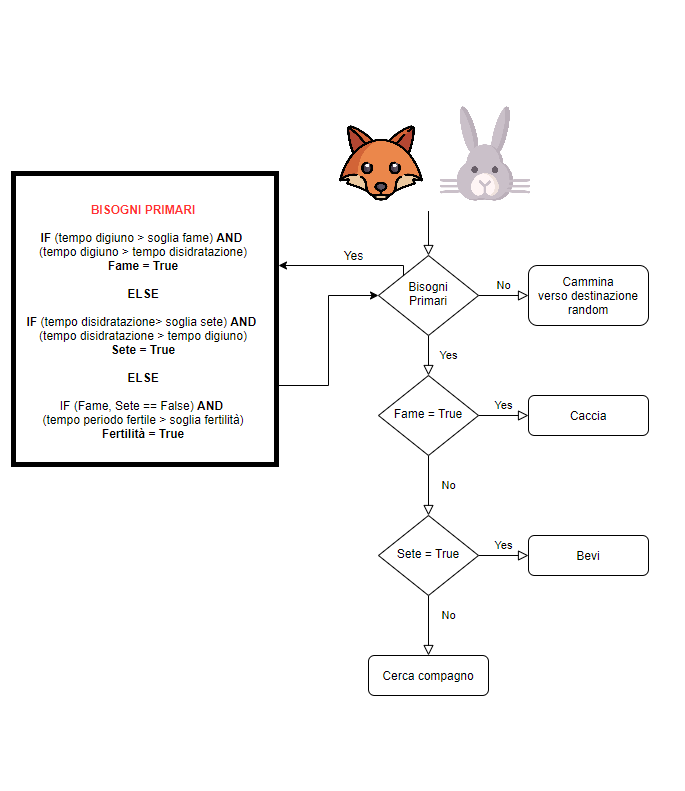
\includegraphics[scale = 0.7]{diagramma_comportamentale.png}
     \label{fig:diagrammaComportamentale}
     \caption{Il diagramma in figura mostra il comportamento degli agenti di tipo Volpe e di tipo Coniglio ad ogni iterazione.}
\end{figure}

\subsubsection{Procedura Caccia}
\label{sec:Caccia}
La procedura denominata \emph{Caccia} permette ai Conigli di cercare carote nelle vicinanze per potersi sfamare e permette alle volpi di cercare dei conigli nelle vicinanze in modo tale da poterli cacciare per poter soddisfare la propria necessità di cibarsi.
Come visibile nella figura \ref{fig:diagrammaCaccia}, l'agente per prima cosa cerca se c'è una preda nell'area circolare avente come centro la posizione attuale dell'agente e come raggio la sua percezione. Si noti che per i cuccioli e per gli anziani (ovvero quelle volpi e quei conigli che hanno età inferiore a 0.5 o superiore a 4) la loro percezione viene dimezzata. Se l'agente non trova una preda (una carota nel caso dei conigli, un coniglio nel caso delle volpi), allora esso camminerà verso un punto posizionato in modo casuale nell'ambiente e al prossimo istante temporale verranno eseguite le valutazioni e le conseguenti azioni descritte precedentemente e mostrate nella figura \ref{fig:diagrammaComportamentale}. 
Viceversa, nel caso in cui l'agente ha trovato una preda nei dintorni, allora l'ambiente comunica all'agente se la preda è ancora viva oppure no. Quest'ultima valutazione si rende utile per evitare il presentarsi di alcuni conflitti che occorrerebbero nel momento in cui un agente ha trovato una preda, ma prima che esso possa raggiungerla, un altro agente se ne ciba rendendola non più disponibile per il primo agente.
Nel caso in cui la preda non dovesse essere più presente nell'ambiente, allora l'agente si muove verso una destinazione random e ripete dall'inizio la procedura. Invece, nel caso in cui la preda dovesse essere ancora viva, l'agente inizia a correre verso la preda. Si noti che la velocità di corsa dei cuccioli e degli anziani è dimezzata rispetto a quella degli agenti adulti. Nel momento in cui la preda risulterà essere ad una distanza ridotta (inferiore a 5 pixel), allora la preda verrà uccisa, il parametro \emph{fame} dell'agente viene posto a False e l'attributo \emph{tempo\_digiuno}, che indica il tempo trascorso dall'ultima volta che l'agente ha mangiato, viene settato con un valore pari a zero. Se invece la distanza dovesse essere superiore a 5 pixel, l'agente chiede all'ambiente se la preda è ancora viva e la procedura si ripete. 

\begin{figure}
     \centering
     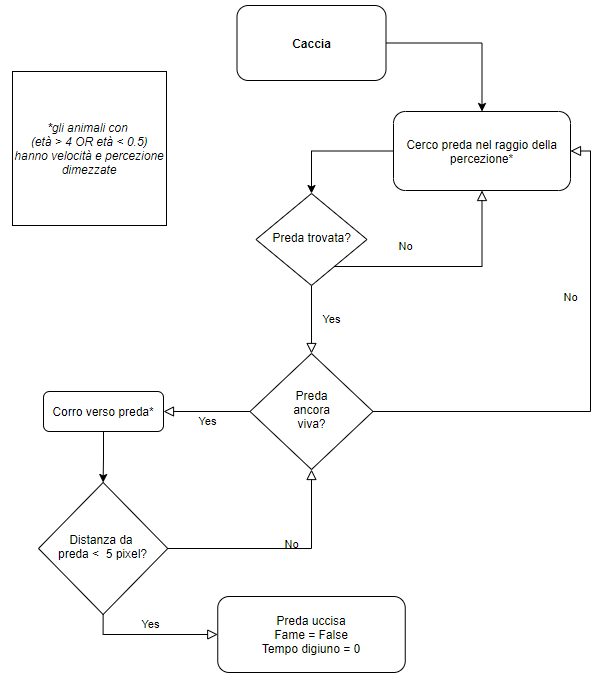
\includegraphics[scale = 0.7]{Caccia.png}
     \label{fig:diagrammaCaccia}
     \caption{Il diagramma in figura mostra come si comportano i conigli e le volpi quando hanno la necessità di cibarsi}
\end{figure}

\subsubsection{Procedura Bevi}
\label{sec:Bevi}
L'operazione denominata \emph{Bevi} è stata implementata come descritto nella figura \ref{fig:diagrammaBevi}. 
\begin{figure}
     \centering
     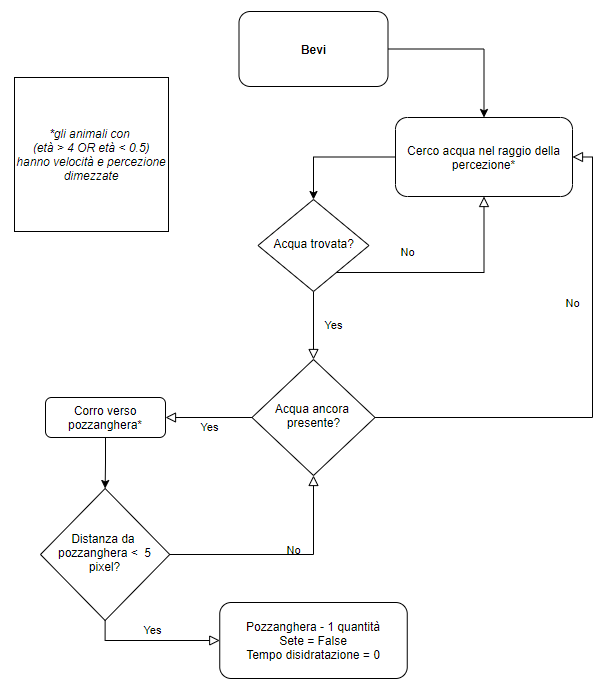
\includegraphics[scale = 0.7]{Sete.png}
     \label{fig:diagrammaBevi}
     \caption{Il diagramma in figura mostra come si comportano i conigli e le volpi quando hanno la necessità di dissetarsi}
\end{figure}
La procedura prevede in primo luogo che l'agente cerchi una pozzanghera nell'area circolare avente come centro la posizione attuale dell'agente e come raggio la percezione dell'agente stesso. Si noti che anche in questa situazione valgono le considerazioni di cui sopra: i cuccioli (età minore di 0.5) e gli anziani (età superiore a 4) hanno valori di percezione e velocità dimezzate rispetto a quelle degli adulti. Se l'ambiente comunica all'agente che non esiste una pozzanghera nei dintorni, allora l'agente si muove con destinazione casuale nell'ambiente e dal prossimo istante temporale ripeterà il ciclo di valutazioni descritte precedentemente e mostrate nella figura \ref{fig:diagrammaComportamentale}. Viceversa, nel caso in cui l'ambiente comunica all'agente che esiste una pozzanghera nelle vicinanze, allora l'agente inizia a correre verso la posizione della pozzanghera. In ogni istante temporale l'ambiente comunica all'agente se la pozzanghera è ancora presente nell'ambiente o meno (potrebbe accadere che altri agenti nel frattempo si sono diretti verso la stessa direzione e abbiano esaurito la pozzanghera). In caso negativo l'agente si dirige camminando verso una destinazione casuale e nel successivo istante temporale ripete la procedura dall'inizio. Se invece l'ambiente comunica all'agente che la pozzanghera non è stata esaurita da altri agenti, allora esso continua la corsa verso di essa. Questo ciclo si ripete fino a quando la distanza tra la pozzanghera e l'agente risulta essere inferiore a 5 pixel. In questa situazione l'agente si disseta, quindi il valore dell'attributo \emph{sete} diventa False, viene diminuita di una unità la dimensione della pozzanghera (che inizialmente ha una dimensione pari a 3) e l'attributo \emph{tempo\_disidratazione} dell'agente che identifica il tempo trascorso dall'ultima volta che si è abbeverato viene impostato con un valore pari a zero. 

\subsubsection{Procedura Cerca compagno}
\label{sec:Accoppiamento}
La procedura di ricerca di un compagno, di accoppiamento e di riproduzione viene illustrata nella figura \ref{fig:diagrammaAccoppiamento}. 
\begin{figure}
     \centering
     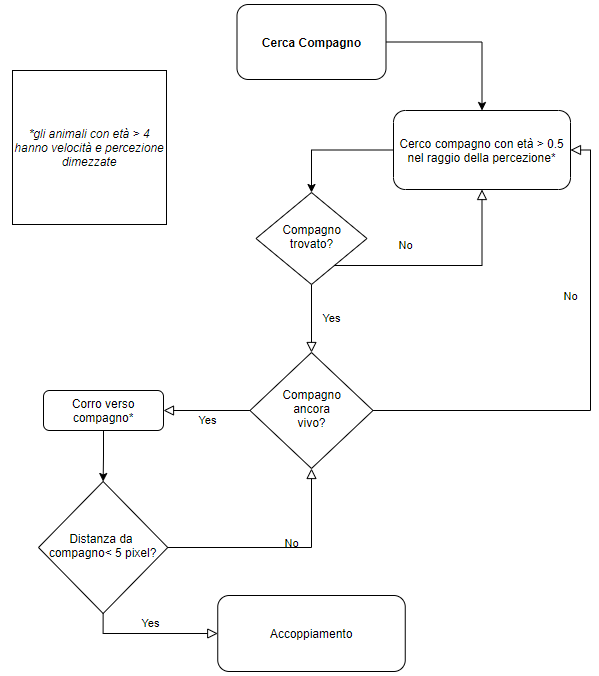
\includegraphics[scale = 0.7]{Cerca_Compagno.PNG}
     \label{fig:diagrammaAccoppiamento}
     \caption{Il diagramma in figura mostra come si comportano i conigli e le volpi quando hanno la necessità di accoppiarsi}
\end{figure}
Per prima cosa ogni agente che ha la necessità di accoppiarsi chiede all'ambiente se ci sono altri agenti dello stesso tipo e con età maggiore di 0.5 (i cuccioli non si possono accoppiare) nell'area circolare centrata nella posizione attuale dell'agente e di raggio pari alla percezione dello stesso.
In caso negativo l'agente si muove verso una direzione casuale nell'ambiente e riprende l'esecuzione delle operazioni descritte nella figura \ref{fig:diagrammaComportamentale}. Viceversa, in caso affermativo l'ambiente comunica la posizione del candidato compagno più vicino. L'agente inizia a correre verso la posizione comunicatagli dall'ambiente e in ogni istante temporale chiede all'ambiente se il compagno è ancora vivo. In caso negativo esso si sposta verso una destinazione casuale per poi ripetere l'intera procedura. Se invece, l'ambiente comunica che il compagno è ancora vivo, allora l'agente continua la corsa verso di esso. Questa operazione viene continuamente ripetuta in ogni istante temporale fino a quando la distanza tra i due agenti risulta essere inferiore a 5 pixel. In questo caso l'accoppiamento può avere luogo. 

L'accoppiamento viene gestito in questo modo: gli attributi \emph{fertilita} dei due agenti coinvolti nell'accoppiamento vengono impostati a False, gli attributi \emph{tempo\_periodo\_fertile}, che indicano quanto tempo è passato dall'ultimo accoppiamento dell'agente, vengono posti a 0 e inoltre l'attributo \emph{gravidanza} di uno dei due agenti viene impostato a True. Oltre a ciò, dopo un periodo di gestazione, avviene la nascita  dei cuccioli(vedere la sezione \ref{sec:tuning} per informazioni relative al numero di cuccioli che nascono ad ogni parto e ai tempi di gestazione delle due tipologie di agenti). Nelle versioni del modello che non prevedono la gestione dell'evoluzione genetica i parametri \emph{soglia\_fame}, \emph{soglia\_morte\_di\_fame}, \emph{soglia\_sete}, \emph{soglia\_morte\_di\_sete}, \emph{soglia\_fertilità}, \emph{percezione}, \emph{velocita\_camminata} e \emph{velocita\_corsa} dei cuccioli vengono impostati seguendo il seguente principio: 
\[
    y = rand(min(x_1, x_2), max(x_1, x_2))
\]
Dove $x$ è il valore ereditato dal cucciolo e $x_1$ e $x_2$ sono i rispettivi parametri dei due genitori.  Viceversa, nella versione del modello in cui è stata implementata l'evoluzione genetica,
ogni qualvolta nasce un cucciolo i parametri \emph{soglia\_fame}, \emph{soglia\_morte\_di\_fame}, \emph{soglia\_sete}, \emph{soglia\_morte\_di\_sete}, \emph{soglia\_fertilità}, \emph{percezione}, \emph{velocita\_camminata} e \emph{velocita\_corsa} dei cuccioli vengono ereditati dai genitori seguendo questo approccio:
\[
    y = rand(min(x_1, x_2), max(x_1, x_2)) + rand(-y1, y1) 
\]
Dove $y$ è il parametro ereditato dal cucciolo e $x_1, x_2$ sono i rispettivi parametri dei due genitori. Invece, $y_1$ è un offset appositamente scelto per ognuno degli otto parametri. Un valore grande implica che i cambiamenti genetici, anche nel breve periodo, siano più ampi, mentre se viene scelto un valore basso i cambiamenti genetici, almeno nel breve periodo,  risultano essere piuttosto contenuti. 
\end{comment}

\clearpage
\section{Ambiente di sviluppo e Codice}
\label{sec:codice}
Al fine di realizzare il progetto di simulazione, si è deciso di utilizzare il linguaggio di programmazione python, sfruttando la libreria pygame per realizzare l'interfaccia grafica. Pygame, come descritto nel sito ufficiale\cite{PyGame}, è un modulo python pensato per lo sviluppo di videogiochi che aggiunge funzionalità alla libreria multi-piattaforma SDL. Il suo utilizzo non è limitato esclusivamente allo sviluppo di videogame, ma anche per realizzare simulazioni multi-agente come nel caso del progetto corrente. Dal lato dello sviluppo si è suddiviso il codice in diversi moduli, per garantirne una migliore chiarezza e flusso di esecuzione, e si sono utilizzate diverse librerie:
\begin{itemize}
    \item \textit{\textbf{random}} per la gestione della simulazione è stato fatto un ampio utilizzo della generazione di valori pseudocasuali, attraverso questa libreria ed in particolare del metodo $randint(int_1, int_2)$, per ricreare al meglio la variabilità e l'entropia di un sistema complesso quale un ecosistema, memorizzando ad ogni esecuzione il \textbf{seed} per poterla rieseguire.
    
    \item \textbf{\textit{pandas}} per la gestione dei dati attraverso l'utilizzo di dataframe e per la memorizzazione in file \textit{.csv} per effettuarne lo studio.
    
    \item \textbf{\textit{matplotlib}} per la creazione dei grafici.
    
    \item \textbf{\textit{\textit{os}}} e \textbf{\textit{sys}} per l'interfacciamento con il sistema operativo: gestione evento chiusura finestra, creazione cartelle e memorizzazione file.
    
\end{itemize} 

Il codice, separato in vari moduli, è così suddiviso: \begin{itemize}
    \item \textbf{Simulazione}: modulo principale in cui si effettua la simulazione vera e propria. Qui sono descritti i vari agenti come classi e viene utilizzata l'ereditarietà per rappresentare gli agenti Volpe e Coniglio, ereditando alcuni parametri comuni dalla superclasse Animale. Viene inoltre gestita la raccolta dei dati, memorizzando delle “fotografie” dello stato della simulazione ad ogni 250 iterazioni, e tutto ciò che riguarda il "game loop", ovvero la logica con cui pygame gestisce le iterazioni. Anche il tempo di esecuzione è gestito in questo modulo e viene calcolato sulla base del lasso temporale che passa da un'iterazione e l'altra e serve per regolare la quantità di pixel che ogni agente percorre in movimento. Ad ogni 500 iterazioni un controllo va a gestire il cambio delle stagioni e ciò che ne comporta, come il cambio di render del terreno e di diversi parametri di gestione della pioggia e delle carote. Una volta chiusa la finestra di simulazione questo modulo salverà i dati e li passerà al modulo \textit{Plot}. All'inizio dell'esecuzione si utilizzeranno diversi parametri per regolare il funzionamento e la visualizzazione della simulazione. Essi sono:
    \begin{itemize}
        \item \textbf{GRAFICA}: se a \textit{True} verranno visualizzati gli agenti animali con sprite 2D, se a \textit{False} gli agenti animali saranno dei pixel, garantendo una migliore fluidità nell'esecuzione nel caso si vada ad effettuare una simulazione con molti render di agenti su schermo;
        \item \textbf{EVOLUZIONE:} se a \textit{True} nella riproduzione si sommerà un offset casuale ai parametri degli agenti per andare a studiare il meccanismo di selezione evolutiva dei geni, se a \textit{False} la riproduzione genererà animali con parametri ereditati dai genitori senza possibilità di mutamento.
        \item \textbf{REINSERIMENTO:} se a \textit{True} ogni cambio di stagione verranno reinseriti alcuni animali, se a \textit{False} non ci sarà reinserimento. Utile per andare a studiare l'ambiente come sistema chiuso o aperto.
        \item \textbf{NUMERO CONIGLI/VOLPI/POZZANGHERE/CAROTE:}  rappresenta il numero di agenti che verranno inizializzati ad inizio dell’esecuzione.
        \item \textbf{PROBABILITA CRESCITA CAROTE:}  rappresenta la probabilità che ha ogni carota, ad ogni iterazione, di generare un’altra carota vicino ad essa. 
        \item \textbf{QUANTITA ACQUA:}  rappresenta il numero di animali che può dissetarsi da una singola pozzanghera.
        \item \textbf{WIDTH/HEIGHT:}  rappresentano la dimensione della finestra di visualizzazione della simulazione, cambiarli non modifica solo l’aspetto visivo ma va ad alterare anche l’esito della simulazione stessa a causa delle distanze ridotte tra gli agenti.

    \end{itemize}
    
    \item \textbf{Ambiente:} modulo inizializzato all'interno di \textit{Simulazione} che gestisce e regola l'ambiente della simulazione. Al suo interno sono memorizzati i metodi per aggiungere, rimuovere, processare ed effettuare il render degli agenti. Al suo interno vi sono inizializzate alcune variabili fondamentali ai fini della simulazione, come:
    \begin{itemize}
\item  Il numero di animali nati e morti dall’inizio dell’esecuzione;
\item I giorni e le stagioni;
\item La lista degli agenti che verranno aggiunti e rimossi alla prossima iterazione.
\end{itemize}

    \item \textbf{Vector2D}: collezione di metodi per la gestione delle coordinate e dello spazio vettoriale. Vengono utilizzati metodi per ottenere ed elaborare la posizione, la distanza, il modulo (magnitudine), la norma e la direzione dei punti sul piano 2D.
    
    \item \textbf{Plot}: modulo che prende come parametro il file \textit{.csv} generato dalla simulazione e ne visualizza i valori creando diversi grafici e memorizzandoli in cartelle apposite, identificate dal seed della simulazione e la presenza di evoluzione (tag E) e reintroduzione (tag R).
\end{itemize}

\begin{comment}
\section{Tuning dei parametri}
\label{sec:tuning}
Una delle fasi più delicate dell'intero progetto è stata quella dedicata al tuning dei molti parametri che compongono il modello. Questa operazione in generale è fondamentale per far si che il comportamento del modello sia conforme rispetto al fenomeno reale che si intende simulare. In letteratura esiste una grande varietà di tecniche altamente sofisticate atte all'ottimizzazione dei parametri di modelli complessi. Tuttavia in questo progetto si è deciso di seguire un approccio molto più semplice. Per quanto concerne i parametri vitali degli animali coinvolti nella simulazione si è cercato di tener fede ai dati reali. Per esempio sono stati reperiti dati da varie fonti dati riguardanti i tempi di gestazione, il numero di cuccioli che mediamente nascono ad ogni parto per ciascuna delle due specie ecc. in modo tale che il modello fosse aderente alla realtà. Altri parametri, come la velocità di camminata, la velocità di corsa ecc. di cui non è stato possibile reperire dati affidabili, sono stati stimati e opportunamente impostati in seguito all'esecuzione di svariate run del modello in modo tale che il comportamento dello stesso fosse il più realistico possibile. I valori finali scelti per ogni parametro e il relativo processo decisionale sono descritti qui di seguito.

\begin{itemize}
    \item Numero iniziale di agenti da includere nel modello. La valutazione relativa al setting ideale di questi parametri ha considerato la necessità di bilanciare al meglio il numero di agenti affinché il sistema risultasse il più stabile possibile. Uno sbilanciamento totale di questi parametri infatti avrebbe prodotto come effetto l'estinzione prematura di una o più di una delle categorie di agenti coinvolti. Per esempio, fissare un numero molto elevato di conigli e uno basso di carote presenti nel sistema all'inizio della simulazione avrebbe prodotto come effetto la completa estinzione in breve tempo dei conigli che sarebbero tutti precocemente morti di fame. Analogamente, fissare un numero di pozze d'acqua ridotto rispetto al numero di conigli e volpi avrebbe prodotto come effetto quello della completa estinzione di entrambi i tipi di animali. 
    In conclusione, i valori finali scelti sono i seguenti:
    \begin{itemize}
        \item \textbf{Conigli}: 75
        \item \textbf{Volpi}: 25
        \item \textbf{Acqua}: 200
        \item \textbf{Carote}: 250
    \end{itemize}
    \item \textbf{Dimensione dell'ambiente}. Si è constatato in seguito a diverse prove, che la dimensione dell'ambiente in rapporto al numero di agenti che lo popolano non deve essere troppo elevata. La ragione di questo è relativa al fatto che se l'ambiente fosse troppo grande, allora gli agenti si disperderebbero al suo interno. Ciononostante è altresì essenziale che la dimensione dell'ambiente non sia eccessivamente ridotta in proporzione al numero di agenti al suo interno e alla loro velocità di movimento. In seguito a tali valutazioni, si è optato per adottare i seguenti valori: 1200x800 pixel.
    \item \textbf{Clock tick}. Questo parametro indica con quale velocità il tempo scorre nella simulazione. Un valore elevato implica che il tempo trascorra con una velocità elevata, un valore basso implica che il tempo trascorra con una velocità moderata. Per far sì che il movimento e il comportamento degli agenti sia comprensibile a chi guarda la simulazione si è ritenuto giusto optare per un valore pari a 150. 
    \item \textbf{Probabilità pioggia in primavera}. Questo valore indica con quale probabilità in ogni istante temporale cadrà della pioggia. Questo parametro è strettamente legato alla frequenza delle piogge nella stagione primaverile: un valore alto indica il fatto che le piogge sono frequenti, un valore basso indica che le piogge sono scarse. Il valore è scelto è pari a   
    \item \textbf{Quantità pozzanghere aggiunte in primavera}. Questo parametro indica, per ogni istante temporale, in caso di pioggia quante pozzanghere d'acqua verranno aggiunte all'ambiente. Si è optato per usare un valore pseudocasuale compreso tra 0 e 10. 
    \item \textbf{Probabilità aggiunta carote in primavera}. Indica la probabilità di aggiungere una carota ad ogni step temporale durante la primavera. Si è optato per un valore pari a 33\%. Così facendo in ogni step temporale in primavera c'è il 33\% di possibilità che venga aggiunta una carota nell'ambiente. La posizione di questo nuovo agente aggiunto è definita in modo casuale. 
    \item \textbf{Probabilità pioggia in estate}. Analogamente al valore speculare relativo all'estate, indica con quale probabilità in ogni istante temporale in estate si presenti la pioggia. Il valore scelto per questo parametro è pari a 
    \item \textbf{Quantità pozzanghere aggiunte in estate}. Indica quante pozzanghere in estate in caso di pioggia vengono aggiunte all'ambiente. Si è optato per un valore casuale compreso tra x e y.
    \item \textbf{Probabilità aggiunta carote in estate}. Indica ad ogni istante temporale in estate qual è la probabilità con cui verrà aggiunta una carota nell'ambiente. Il valore scelto è pari a x\%. 
    \item \textbf{Probabilità pioggia in autunno}. Si è optato per un valore pari a z \% poiché la frequenza delle piogge in autunno in genere è maggiore di quella delle piogge in estate e paragonabile a quella delle piogge in primavera.
    \item \textbf{Quantità pozzanghere aggiunte in autunno}. Si è optato per un valore casuale compreso tra x e y, poiché in linea del tutto generale in autunno le piogge sono più frequenti, ma meno intense rispetto ai temporali estivi che quindi formano un numero minore di pozzanghere nell'ambiente. 
    \item \textbf{Probabilità aggiunta carote in autunno}.  Il valore scelto è pari a x\%, poiché le carote si sviluppano più frequentemente in estate piuttosto che in autunno.
    \item \textbf{Probabilità pioggia in inverno}. Si è optato per un valore pari a z \% poiché la frequenza delle piogge in inverno in genere è maggiore di quella delle piogge in estate e paragonabile a quella delle piogge in primavera e in autunno.
    \item \textbf{tempo di gestazione delle volpi}. Il tempo di gestazione della volpe rossa in natura è compreso tra i 49 e i 58 giorni \cite{VolpeGestazione}. Si è impostato tale parametro in modo che assumesse un valore casuale compreso tra i 30 e i 40 istanti temporali. 
    \item \textbf{Tempo di gestazione dei conigli}. La durata della gestazione del coniglio selvatico europeo è pari a 30 giorni\cite{WikiConiglio}. Per mantenere corretta la proporzione tra i tempi di gestazione delle volpi e quelle dei conigli nel modello, si è optato per impostare questo parametro in modo tale che assumesse un valore casuale compreso tra i 18 e i 24 istanti temporali. 
    \item \textbf{Nascite delle volpi}. La volpe rossa in media partorisce dai 3 ai 5 cuccioli \cite{WikiVolpe}. Si è deciso di mantenere invariato questo aspetto anche nel modello: ogni qualvolta una volta una volpe si riproduce da origine ad un numero casuale compreso tra 3 e 5 cuccioli.
    \item \textbf{Nascite dei conigli}. Ogni coniglio da alla luce un numero compreso tra i 3 e i 14 cuccioli\cite{WikiConiglio}. Nel modello si è impostato tale parametro in modo che assumesse un valore casuale compreso tra 3 e 9, poiché dopo varie esecuzioni delle simulazioni si è giunti alla conclusione che settando tale parametro in modo che assumesse valori compresi tra 3 e 9, il numero di conigli aumenterebbe in modo esponenziale, rendendo il modello instabile. 
    \item \textbf{Aspettativa di vita delle volpi}. In natura mediamente le volpi vivono fino agli 8 anni\cite{WildLifeFox}. Il parametro relativo all'età raggiunta la quale la volpe muore di vecchiaia è stato fissato ad un valore pari a 4.5. Ad ogni istante temporale l'età di ogni agente viene incrementata di un valore pari a 0,003. Questo significa che ogni volpe muore di vecchiaia dopo che sono passati 1500 step temporali dalla sua nascita.
    \item \textbf{Aspettativa di vita dei conigli}. L'aspettativa di vita di un coniglio selvatico in natura è pari circa a 9 anni. Per far si che il parametro relativo all'aspettativa di vita dei conigli e quello relativo all'aspettativa di vita delle volpi fossero proporzionati rispetto alla realtà è stato fissato un valore di aspettativa di vita pari a 5 per i conigli. 
    \item \textbf{Giovinezza di volpi e conigli}. Quando le volpi e i conigli sono ancora cuccioli la loro percezione viene gestita in modo tale che sia pari alla metà della percezione media degli stessi animali in età adulta. Inoltre, volpi e conigli cuccioli non hanno la necessità di riprodursi. Volpi e conigli vengono considerati cuccioli fino a quando la loro età sarà inferiore a 0.5. 
    \item \textbf{Vecchiaia di volpi e conigli}. Le volpi e i conigli vengono considerati anziani quando la loro età supera il valore pari a 4. 
    \item \textbf{Soglia fame Coniglio}. Questo parametro per ogni agente di tipo Coniglio presente all'inizio della simulazione è pari a $x = rand(200, 250)$. 
    \item \textbf{Soglia morte di fame Coniglio}. Si è scelto un valore pari a $x=rand(500, 600)$ per tutti i Conigli presenti all'inizio della simulazione. 
    \item \textbf{soglia sete Coniglio}. Il valore scelto per i conigli presenti all'inizio della simulazione è pari a $x=rand(200, 250)$.
    \item \textbf{soglia morte di sete Coniglio}. Il valore scelto per i conigli presenti all'inizio della simulazione è pari a $x=rand(500, 600)$.
    \item \textbf{soglia fertilità Coniglio}. Si è optato per il seguente valore $x=rand(250, 300)$. 
    \item \textbf{soglia percezione Coniglio}. Il valore iniziale scelto è pari a $x= rand(15, 20)$.
    \item \textbf{soglia velocità camminata Coniglio}. Il valore iniziale per questo parametro è stato impostato pari a $x=rand(40, 60)$.
    \item \textbf{soglia velocità corsa Coniglio}. Il valore iniziale di questo parametro è pari a $x=rand(65, 75)$.
    \item \textbf{Soglia fame Volpe}. Si è optato per il seguente valore iniziale: $x=rand(200, 250)$ in modo tale che i conigli e le volpi iniziassero a percepire la fame nello stesso istante a parità di condizioni. 
    \item \textbf{Soglia morte di fame Volpe}. Si è optato per il seguente valore iniziale $x=rand(550, 650)$. Questo implica che le volpi, almeno nelle prime fasi della simulazione quando gli effetti dell'evoluzione genetica non si sono ancora manifestati, possono resistere leggermente più tempo senza mangiare rispetto ai conigli.  
    \item \textbf{soglia sete Volpe}. Il valore scelto è pari a $x=rand(200, 250)$ ovvero il medesimo valore scelto per gli agenti di tipo Coniglio. 
    \item \textbf{soglia fertilità Volpe}. Si è optato per il seguente valore: $x=rand(500, 600)$. In questo modo le volpi si riproducono molto meno di frequente così come effettivamente accade in natura. Infatti in natura le volpi si riproducono mediamente una volta all'anno\cite{VolpeGestazione}, mentre i conigli si riproducono più volte all'anno\cite{WikiConiglio}.
    \item \textbf{soglia percezione Volpe}. Si è optato per il medesimo valore utilizzato per i Conigli: $x=rand(15, 20)$. 
    \item \textbf{soglia velocità camminata Volpe}. Anche in questo caso si è scelto lo stesso valore dei Conigli pari a $x=rand(40, 60)$.
    \item \textbf{soglia velocità corsa Volpe}. Anche per quest'ultimo parametro si è adottato il medesimo valore utilizzato per i Conigli, pari a $x=rand(65, 75)$.
\end{itemize}
\end{comment}
\section{Validazione}

\section{Analisi dei risultati}

\section{Conclusioni e sviluppi futuri}






\newpage
\printbibliography	
\end{document}
